\documentclass[aps,prx,twocolumn,superscriptaddress,amsmath]{revtex4-2}
\usepackage[hidelinks]{hyperref}
\usepackage[separate-uncertainty=true,binary-units]{siunitx}
\usepackage{graphicx}
\usepackage{tikz}
\usepackage{glossaries}
\usepackage{ifthen}
\usepackage[noabbrev,capitalise]{cleveref}
\usepackage{import}
\usepackage{rotating}
\usepackage[T1]{fontenc}

\usetikzlibrary{
	calc,
	shapes,
	positioning,
	backgrounds,
	decorations.pathreplacing,
	fit,
	external,
	fadings}
%\tikzexternalize

\pgfdeclarelayer{background}
\pgfdeclarelayer{foreground}
\pgfsetlayers{background,main,foreground}

\definecolor{nicegray}{HTML}{555555}
\definecolor{nicered}{HTML}{AF5A50}
\definecolor{niceblue}{HTML}{005B82}
\definecolor{nicegreen}{HTML}{7D966E}
\definecolor{niceyellow}{HTML}{D7AA50}

% Custom abbreviations for cleveref
\crefname{figure}{FIG.}{FIG.}
\crefname{table}{TABLE}{TABLE}
\crefname{equation}{Eq.}{Eq.}
\crefname{supp}{SI}{SI}

% Define abbreviations
\newacronym{ei}{E-I}{excitatory-inhibitory}
\newacronym{lif}{LIF}{leaky integrate-and-fire}
\newacronym{asic}{ASIC}{application-specific integrated circuit}
\newacronym{ppu}{PPU}{plasticity processing unit}
\newacronym{simd}{SIMD}{single instruction multiple data}
\newacronym{hmm}{HMM}{Hidden Markov Model}
\newacronym{psp}{PSP}{post-synaptic potential}
\newacronym{epsp}{EPSP}{excitatory post-synaptic potential}

\begin{document}


\title{Autocorrelations from emergent bistability in homeostatic spiking neural networks on neuromorphic hardware}
\author{Benjamin Cramer}
\author{Markus Kreft}
\author{Sebastian Billaudelle}
\author{Vitali Karasenko}
\author{Aron Leibfried}
\author{Eric Müller}
\author{Philipp Spilger}
\author{Johannes Weis}
\author{Johannes Schemmel}
\affiliation{Kirchhoff-Institute for Physics, Im Neuenheimer Feld 227, Heidelberg University, Germany}
\author{Miguel A. Mu\~noz}
\affiliation{Departamento de Electromagnetismo y Física de la Materia e Instituto Carlos I de Física Teórica y Computacional, Universidad de Granada, E-18071 Granada, Spain}
\author{Viola Priesemann}
\affiliation{Max Planck Institute for Dynamics and Self-Organization, Am Fa{\ss}berg 17, 37077 G\"ottingen, Germany}
\affiliation{Institute for the Dynamics of Complex Systems, University of G\"ottingen, Friedrich-Hund-Platz 1, 37077 G\"ottingen, Germany}
\author{Johannes Zierenberg}
\affiliation{Max Planck Institute for Dynamics and Self-Organization, Am Fa{\ss}berg 17, 37077 G\"ottingen, Germany}

\date{\today}

\begin{abstract}

A fruitful approach towards neuromorphic computing is to mimic mechanisms of the brain in physical devices, which led to successful replication of neuron-like dynamics and learning in the past.
However, there remains a large set of neural self-organization mechanisms whose role for neuromorphic computing has yet to be explored.
One such mechanism is homeostatic plasticity, which has recently been proposed to play a key role in shaping network dynamics and correlations.
Here, we study --- from a statistical-physics point of view -- the emergent collective dynamics in a homeostatically-regulated neuromorphic device that emulates a network of excitatory and inhibitory \acrlong{lif} neurons.
Importantly, homeostatic plasticity is only active during the training stage and results in a heterogeneous weight distribution that we fix during the analysis stage.
We verify the theoretical prediction that reducing the external input in a homeostatically regulated neural network increases temporal correlations, measuring autocorrelation times exceeding $\SI{500}{\milli\second}$, despite single-neuron timescales of only $\SI{20}{\milli\second}$, in both experiments on neuromorphic hardware and in computer simulations.
However, unlike theoretically predicted near-critical fluctuations, we find that temporal correlations can originate from an emergent bistability.
We identify this bistability as a fluctuation-induced stochastic switching between metastable active and quiescent states in the vicinity of a non-equilibrium phase transition.
Our results thereby constitute a new, complementary mechanism for emergent autocorrelations in networks of spiking neurons with implications for future developments in neuromorphic computing.


%A fruitful approach towards neuromorphic computing is to mimic mechanisms of the brain in physical devices, which led to successful replication of neuron-like dynamics and learning.
%However, there remains a large set of neural self-organization mechanisms whose role for neuromorphic computing is yet to be explored.
%One such mechanisms is homeostatic plasticity, which has recently been proposed to play a key role in shaping network dynamics and correlations.
%Here, we study the emergent collective dynamics in a homeostatic neuromorphic device, emulating a network of excitatory and inhibitory \acrlong{lif} neurons, from a statistical-physics point of view.
%Importantly, homeostatic plasticity is only active during the training stage, resuling in a heterogeneous but fixed weight distribution during the analysis stage.
%We reproduce the theoretical prediction that lowering the external input increases temporal correlations, measuring in both experiments on neuromorphic hardware and in computer simulations autocorrelation times exceeding $\SI{500}{\milli\second}$ despite single-neuron timescales of only $\SI{20}{\milli\second}$, which is compatible with those observed in the living brain.
%However, different to the theoretically predicted close-to-critical fluctuations, we find that temporal correlations can originate from an emergent bistability.
%%A unique feature of neuromorphic computing is that memory is an implicit part of processing through traces of past information in the system's collective dynamics.
%%The extent of memory about past inputs is commonly quantified by the autocorrelation time of collective dynamics.
%%Based on past experimental evidence, a potential explanation for the underlying autocorrelations are close-to-critical fluctuations.
%%Here, we show for self-organized networks of excitatory and inhibitory \acrlong{lif} neurons that autocorrelations can originate from emergent bistability upon reducing external input strength.
%We identify this bistability as a fluctuation-induced stochastic switching between metastable active and quiescent states in the vicinity of a non-equilibrium phase transition.
%%
%%Our results provide  verification of biologically compatible autocorrelation times in networks of \acrlong{lif} neurons, which here are not generated by close-to-critical fluctuations but by emergent bistability in homeostatically regulated networks.
%Our results thereby constitute a new, complementary mechanism for emergent autocorrelations in networks of spiking neurons, with implications for biological and artificial networks

%There is rising experimental evidence that networks of spiking neurons can exhibit emergent autocorrelations that are associated with their information processing capacities.
%However, autocorrelation times as large as in experiments have so far not been reproduced for networks of \acrlong{lif} neurons.
%Here, we demonstrate that networks of excitatory and inhibitory \acrlong{lif} neurons, with homeostatic regulation during development, can exhibit increasing autocorrelation times upon decreasing input connections.
%In our experiments on neuromorphic hardware and in computer simulations, we observe autocorrelation times exceeding $\SI{500}{\milli\second}$ despite single-neuron timescales of only $\SI{20}{\milli\second}$.
%These autocorrelations can be attributed to emergent bistable population activity as a result of fluctuation-induced stochastic switching between metastable active and quiescent states in the vicinity of a non-equilibrium phase transition.
%Our results present
%    (i) a new mechanism for emergent autocorrelations in networks of spiking neurons,
%    (ii) a new perspective on the origin of so-called up-and-down states, and
%    (iii) a general paradigm of fluctuation-induced bistability for driven systems with absorbing states.
%This is a first step towards a fundamental understanding of emergent collective dynamics for neuromorphic computing with self-organized circuits.
\end{abstract}

\pacs{}
\keywords{bistability}

\maketitle

\glsresetall

\section{\label{sec:introduction}Introduction}

% Neuromorphic computing as context to introduce concept of memory within the dynamics
Neuromorphic computing covers a variety of brain-inspired computers, devices, and models that function fundamentally different to common von-Neumann architectures~\cite{schuman_survey_2017-1, furber_large-scale_2016}.
For instance, one can \emph{emulate} the dynamics of neuron membrane potentials and synaptic currents in analog electronic circuits~\cite{schemmel_modeling_2007, schemmel_wafer-scale_2010, friedmann_demonstrating_2017, moradi_scalable_2018, benjamin_neurogrid_2014}.
In general, the hardware-specific information processing and storage calls for hand-in-hand development of hardware and corresponding algorithms, which can be guided by modern artificial intelligence and neuroscience likewise~\cite{markovic_physics_2020}.
A complementary approach is to build customizable, large-scale neuromorphic architectures that can implement brain-inspired plasticity for self-organization, for instance BrainScaleS~\cite{pehle_brainscales-2_2022} or Loihi~\cite{davies_loihi_2018}.
These devices can exhibit diverse emergent population dynamics that depend, among others, on model parameters, plasticity, or network architecture and that may be useful for future developments in neuromorphic computing.
For instance, emergent temporal correlations imply information integration over time that can be important for understanding sequential input like language, i.e., integrating syllables to words, to sentence to meaning~\cite{hasson_hierarchical_2015, rudelt_embedding_2021, cramer_heidelberg_2022}.
%TODO: Lucas new paper
Understanding emergent timescales in neural networks is thus among the basic prerequisites for designing recurrent neural language processing models from scratch.

%Understanding these emergent dynamics and what controls them is a basic prerequisite for desig 

%Information integration over time can be important for understanding sequential input like language, i.e., integrating szlibils tow orkds, to sentence to meaning. Therefore understanding neural networks like this one is basic prerquisite for designing recurrent neural language processing models from scratch.



%will add to the foundation for future developments in neuromorphic computing.

% Homeostatic plasticity
Recent theoretical and experimental results have emphasized the importance of homeostatic plasticity to shape the timescales of neural population dynamics~\cite{zierenberg_homeostatic_2018, kossio_growing_2018, ma_cortical_2019}.
Homeostatic plasticity is a negative feedback that adapts local neural properties to achieve a stable firing rate~\cite{turrigiano_activity-dependent_1998, turrigiano_homeostatic_2004, turrigiano_homeostatic_2012}.
For homeostatically regulated excitable systems, one can prove analytically that lowering the input strength induces an increase in the recurrent coupling and hence increases the autocorrelation time through close-to-critical fluctuations~\cite{zierenberg_homeostatic_2018, kossio_growing_2018}.
These predictions are consistent with experiments on monocular deprivation, where partial reduction of input initially disrupts population activity before homeostatic plasticity tunes cortical networks back towards criticality~\cite{ma_cortical_2019}.
Moreover, they provide a potential explanation for the experimentally observed increase of autocorrelation time along the hierarchical anatomy of cortex~\cite{murray_hierarchy_2014, hasson_hierarchical_2015, raut_hierarchical_2020, spitmaan_multiple_2020, gao_neuronal_2020, siegle_survey_2021}: timescales are shorter in primary sensory regions and longer in higher-order cortical regions.
In the context of neuromorphic computing, homeostatic plasticity was shown to serve as a guiding principle to tune neuromorphic hardware for optimal task performance~\cite{cramer_control_2020}.

%
However, empirical observations of large, emergent autocorrelations seem to contradict prior theoretical predictions for networks of \gls{ei} \gls{lif} neurons.
While empirical estimates of neural autocorrelation times range from $\mathcal{O}(\SI{10}{ms})$ to $\mathcal{O}(\SI{1}{s})$~\cite{murray_hierarchy_2014, hasson_hierarchical_2015, raut_hierarchical_2020, spitmaan_multiple_2020, gao_neuronal_2020, siegle_survey_2021, wasmuht_intrinsic_2018, cavanagh_reconciling_2018, wilting_operating_2018, wilting_between_2019}, early theories and models of networks of \gls{lif} neurons in an \gls{ei} balanced state \cite{vreeswijk_chaos_1996,renart_asynchronous_2010} predict almost vanishing mean correlations.
Instead, more recent reassessments find conditions under which larger correlations can emerge~\cite{harish_asynchronous_2015, rosenbaum_spatial_2017, mastrogiuseppe_intrinsically-generated_2017, baker_correlated_2019} (see also Ref.~\cite{latham_correlations_2017, dahmen_global_2022} for overviews).
Focusing on temporal correlations, recent developments in dynamic mean-field theory~\cite{ostojic_two_2014, mastrogiuseppe_intrinsically-generated_2017, van_meegen_microscopic_2021} reveal parameter ranges with larger emergent autocorrelation times.
However, these autocorrelation times were still on the order of characteristic times of membrane potential or synaptic current, which are typically $\mathcal{O}(\SI{10}{ms})$, and thus distinctively below the ones observed experimentally.

In this work, we study emergent collective dynamics and autocorrelation times in networks of excitatory and inhibitory \gls{lif} neurons emulated on the BrainScaleS neurmorphic system.
This system provides large flexibility for programmable plasticity rules~\cite{pehle_brainscales-2_2022} and hence allows for homeostatic plasticity during a training phase.
We verify that training with reduced external input strength induces increasing autocorrelation times in the test phase that can be more than 20 times larger than the decay time of the membrane potential of individual units.
Since we are using the BrainScaleS-2 single chip, which is limited to 512 Neurons, we complement our experiments with a numerical finite-size scaling analysis that reveals progressively larger autocorrelation times with increasing system size.
Surprisingly, we find that in our setup autocorrelations are not generated by close-to-critical fluctuations~\cite{zierenberg_homeostatic_2018}, but originate from an emergent bistability in the population firing rate.
To explain this bistability, we derive a simple mean-field theory for driven excitable systems that reveals a fluctuation-induced switching between a metastable active phase and a quiescent phase, reminiscent of so-called \emph{up and down} states in brain networks~\cite{wilson_up_2008,stern_spontaneous_1997,cossart_attractor_2003,hidalgo_stochastic_2012}.
We finish with a discussion of how emergent bistability can affect biological and artificial neural networks, as well as other finite systems with an absorbing-to-active transition that are driven by external noise.





% Memory in neuroscience connected to autocorrelation times

%Empirical work from neurophysiology and neuroimaging suggests that neural circuits implement process memory as active traces of past information~\cite{hasson_hierarchical_2015}.
%One measure of the extend over which information can be accumulated is the processing timescale, which has been related to the autocorrelation time of collective neural dynamics~\cite{murray_hierarchy_2014, hasson_hierarchical_2015}.
%It was found that the autocorrelation time is related to the hierarchical anatomy of cortex~\cite{murray_hierarchy_2014, hasson_hierarchical_2015, raut_hierarchical_2020, spitmaan_multiple_2020, gao_neuronal_2020, siegle_survey_2021}: timescales are shorter in primary sensory regions and longer in higher-order cortical regions.
%In fact, empirical observations of autocorrelation times in neural recordings range from $\mathcal{O}(\SI{10}{ms})$ to $\mathcal{O}(\SI{1}{s})$~\cite{murray_hierarchy_2014, hasson_hierarchical_2015, raut_hierarchical_2020, spitmaan_multiple_2020, gao_neuronal_2020, siegle_survey_2021, wasmuht_intrinsic_2018, cavanagh_reconciling_2018, wilting_operating_2018, wilting_between_2019}.
%This seems to contradict prior theoretical predictions for networks of \gls{ei} \gls{lif} neurons, where early theories and models of networks of \gls{lif} neurons in an \gls{ei} balanced state \cite{vreeswijk_chaos_1996,renart_asynchronous_2010} predict almost vanishing mean correlations, though more recent reassessments found conditions under which much larger correlations can appear~\cite{rosenbaum_spatial_2017, mastrogiuseppe_intrinsically-generated_2017, baker_correlated_2019}, see also Ref.~\cite{latham_correlations_2017, dahmen_global_2022} for an overview.
%Focusing on temporal correlations, recent developments in dynamic mean-field theory~\cite{ostojic_two_2014, mastrogiuseppe_intrinsically-generated_2017, van_meegen_microscopic_2021} reveal parameter ranges with emergent autocorrelation times larger, but still on the order of the characteristic time of the membrane potential, typically $\mathcal{O}(\SI{10}{ms})$, which is still far below the ones observed experimentally.
%
%% self-organization
%This raises the question whether the emergence of large autocorrelation times requires additional mechanisms of self-organization.
%A generic mechanism of neural self-organisation is \emph{homeostatic plasticity}, a negative feedback that adapts local neural properties to achieve a stable firing rate~\cite{turrigiano_activity-dependent_1998, turrigiano_homeostatic_2004, turrigiano_homeostatic_2012}.
%For homeostatically regulated excitable systems, one can prove analytically that lowering the input strength induces an increase in the recurrent coupling and hence in the autocorrelation time through close-to-critical fluctuations~\cite{zierenberg_homeostatic_2018}.
%These predictions are consistent with experiments on monocular deprivation~\cite{ma_cortical_2019} and with the hierarchy of timescales~\cite{murray_hierarchy_2014, hasson_hierarchical_2015, raut_hierarchical_2020, spitmaan_multiple_2020, gao_neuronal_2020, siegle_survey_2021}, and have been applied as a guiding principle to tune neuromorphic hardware for optimal task performance~\cite{cramer_control_2020}.
%However, it so far remains unknown whether close-to-critical fluctuations are responsible for emergent autocorrelations in homeostatic regulated \gls{ei}  networks of \gls{lif} neurons, or whether there could be alternative mechanisms.
%
%homeostatic adaptation
%One way a neural network can self-regulate its dynamics to task requirements is through \emph{homeostatic plasticity}.
%Homeostatic plasticity is a negative feedback that adapts local neural properties to achieve a stable firing rate~\cite{turrigiano_activity-dependent_1998, turrigiano_homeostatic_2004, turrigiano_homeostatic_2012}.
%One can prove analytically for homeostatically regulated excitable systems that lowering the input strength induces an increase in the recurrent coupling and hence in the autocorrelation time through close-to-critical fluctuations~\cite{zierenberg_homeostatic_2018}.
%Despite being a simplified framework, these predictions are consistent with experiments on monocular deprivation~\cite{ma_cortical_2019} and the above noted hierarchy of timescales~\cite{murray_hierarchy_2014, hasson_hierarchical_2015, raut_hierarchical_2020, spitmaan_multiple_2020, gao_neuronal_2020, siegle_survey_2021}.
%Moreover, it has been shown that a comparable mechanism can be exploited to tune a neuromorphic chip, emulating a network of \gls{ei} \gls{lif} neurons subject to a variant of spike-timing dependent plasticity, for optimal task performance~\cite{cramer_control_2020}.
%
% the problem
%However, the empirical observations of large autocorrelation times in neural recordings~\cite{murray_hierarchy_2014, raut_hierarchical_2020, wasmuht_intrinsic_2018, cavanagh_reconciling_2018, kim_strong_2021} seem to contradict prior theoretical predictions for networks of \gls{ei} \gls{lif} neurons.
%Early theories and models of networks of \gls{lif} neurons~ in a \gls{ei} balanced state \cite{vreeswijk_chaos_1996,renart_asynchronous_2010}, predicted almost vanishing mean correlations, though more recent reassessments found conditions under which much larger correlations can appear~\cite{rosenbaum_spatial_2017, mastrogiuseppe_intrinsically-generated_2017, baker_correlated_2019}, see also Ref.~\cite{latham_correlations_2017, dahmen_global_2022} for an overview.
%Focusing on temporal correlations, recent developments in dynamic mean-field theory~\cite{ostojic_two_2014, mastrogiuseppe_intrinsically-generated_2017, van_meegen_microscopic_2021} reveal parameter ranges with emergent autocorrelation times on the order of the characteristic time of the membrane potential.
%Thereby, such theoretically possible autocorrelation times are still far below the ones observed experimentally.

%It is thus necessary to (i) verify that  large autocorrelation times can emerge in networks of \gls{ei} \gls{lif} neurons and to (ii) develop a theoretical understanding of their origin.
%Here, we address these open questions using the experimental setup of a neuromorphic chip with homeostatic plasticity during development.
%We verify that reducing the external input strength induces increasing autocorrelation times that can be more than 20 times larger than the decay time of the membrane potential of individual units.
%We complement our size-constrained experiments with a numerical finite-size scaling analysis that reveals progressively larger autocorrelation times for increasing system sizes.
%Surprisingly, we find that in our case autocorrelations are not generated by close-to-critical fluctuations~\cite{zierenberg_homeostatic_2018}, but originate from an emergent bistability in the population firing rate.
%To explain this bistability, we derive a mean-field theory for driven excitable systems that reveals a fluctuation-induced switching between a metastable active phase and a quiescent phase, reminiscent of so-called \emph{up and down} states in brain networks~\cite{wilson_up_2008,stern_spontaneous_1997,cossart_attractor_2003,hidalgo_stochastic_2012}.
%We finish with a discussion of how emergent bistability can affect biological and artificial neural networks, as well as other finite systems with an absorbing-to-active transition that are driven by external noise.

%Finally, we show that such a bistability leads to a dynamic barrier that can be exploited to discriminate different stimuli of varying strength even much after stimulus offset, paving the way to applications that require implicit working memory.


%To study emergent autocorrelation in homeostatic spiking neural networks, we devise experiments on neuromorphic hardware that due to its acceleration and low energy consumption provide us with a lot of statistics in short time at low energy cost.
%These experiments are confined to the neurorphic hardware with 512 neurons, so that we complement them by a finite-size scaling analysis with increasing system size simulated on high-performance compute clusters for selected parameters.\section{\label{sec:introduction}Introduction}

\section{\label{sec:methods}Model and Methods}

To study emergent collective dynamics in homeostatic neuromorphic devices, we combine experiments on an actual neuromorphic device (BrainScaleS-2), computer simulations, and a phenomenological mean-field theory. In this section, we first describe the basic ingredients of the neuromorphic hardware under consideration (Sec.~\ref{sec:methods}~a), formulate a mathematical model that can be implemented on this hardware (Sec.~\ref{sec:methods}~b), build a computer simulation that reproduces the resulting dynamics (Sec.~\ref{sec:methods}~c), and define relevant observables to study population dynamics (Sec.~\ref{sec:methods}~d).

%%%%%%%%%%%%%%%%%%%%%%%%%%%%%%%%%%%%%%%%%%%%%%%%%%%%%%%%%%%%%%%%%%%%%%%%%%%
%%%%%%%%%%%%%%%%%%%%%%%%%%%%%%%%%%%%%%%%%%%%%%%%%%%%%%%%%%%%%%%%%%%%%%%%%%%
%%%%%%%%%%%%%%%%%%%%%%%%%%%%%%%%%%%%%%%%%%%%%%%%%%%%%%%%%%%%%%%%%%%%%%%%%%%
\paragraph{Neuromorphic hardware.}
\label{sec:brainscale}
BrainScaleS-2~\cite{friedmann_demonstrating_2017,schemmel_accelerated_2022,pehle_brainscales-2_2022} is a mixed-signal neurmorphic architecture that allows to emulate networks of up to $512$ \gls{lif} neurons (\cref{fig:chip}B).
The term \textit{emulation} is used to clearly distinguish between this physical implementation, where each observable has a measurable counterpart on the neuromorphic chip, and standard software \textit{simulations} on conventional hardware (see below).
In particular, neurons are implemented as electrical circuits that emulate \gls{lif} dynamics in a time-continuous and parallel manner.
The system further consists of an array of $256 \times 512$ physically implemented current-based synapses that support near arbitrary topologies.
Their dynamics emulate leaky currents and feature coupling strengths $w_{ij}$ with a precision of \SI{6}{\bit}, i.e., $64$ discrete values, which limits synaptic weights to integers in the range $[0,63]$.
More technical details are provided in \cref{sec:appendix_hardware}.
Due to the analog implementation, time constants are determined by the electrical components on the substrate and are rendered approximately a factor \num{1000} times faster than the ones of their biological archetype.
Within this paper, all referenced time scales are converted to the equivalent biological time domain unless otherwise stated.

Homeostatic plasticity is implemented on-chip by a specialized, freely-programmable processor unit: the \gls{ppu}~\cite{friedmann_demonstrating_2017}.
The \gls{ppu} is able to update the synaptic weights of \SI{128}{} synapses in parallel.
To measure local spike rates relevant for our plasticity rule (see below), we draw on dedicated circuits within each neuron that count the number of emitted spikes.

The system comes with specialized accelerators for the drawing of random numbers~\citep{schemmel_accelerated_2020}.
These facilitate an on-chip generation of Poisson distributed input spikes as well as the efficient implementation of the stochastic homeostatic regulation without additional communication bottlenecks.
The only remaining communication with the host system consists of the transfer of instructions for configuring the BrainScaleS-2 system at the beginning and the readout of the result at the end of an experiment~\citep{muller_extending_2020,muller_scalable_2022}, making the hardware implementation very fast.

The neuromorphic chip is subject to variations both in space and time:
first, the analog implementation causes temporal noise within the model dynamics and second, the production process necessarily leads to small variations across electrical components.
The latter variations can, however, be mitigated by exploiting the configurability of the BrainScaleS-2 system by resorting to calibration routines~\citep{muller_scalable_2022}, thereby reducing the parameter spread across neurons (see \cref{sec:parametrization}).
The remaining variability of parameters can be quantified by their mean and standard deviation (\cref{tab:parameters}).


%%%%%%%%%%%%%%%%%%%%%%%%%%%%%%%%%%%%%%%%%%%%%%%%%%%%%%%%%%%%%%%%%%%%%%%%%%%
%%%%%%%%%%%%%%%%%%%%%%%%%%%%%%%%%%%%%%%%%%%%%%%%%%%%%%%%%%%%%%%%%%%%%%%%%%%
%%%%%%%%%%%%%%%%%%%%%%%%%%%%%%%%%%%%%%%%%%%%%%%%%%%%%%%%%%%%%%%%%%%%%%%%%%%
\paragraph{Neural network model.}
\label{sec:model}
As a minimal model of biological spiking neurons, we consider a recurrent network of $N=512$ (unless otherwise stated) \gls{lif} neurons coupled to an input layer consisting of $N/2$ Poisson sources (\cref{fig:chip}A).
The model is build to reflect the architecture of BrainScaleS-2.
Each \gls{lif} neuron integrates spikes from, on average, $K^\mathrm{rec}=100$ recurrent neurons of the network and from, on average, $K^\mathrm{ext}$ external neurons of the input layer that will be varied to adjust the strength of external input.
The \emph{physical} connection between neuron $i$ and $j$ is randomly realized, $c_{ij}=\{-1,0,1\}$, and further weighted by an integer-value coupling weight $w_{ij}\in[0, 63]$.
Neurons can be either excitatory or inhibitory, which is reflected in the sign of $c_{ij}$ for a given neuron $j$ for all outgoing coupling synapses.
Also, in analogy with cortical networks~\cite{douglas_inhibition_2009}, \SI{20}{\percent} of the neurons in both network and input layer are inhibitory.
While the recurrent neurons are \gls{lif} neurons, input sources generate spikes independently as a Poisson process with rate $\nu^\mathrm{ext}=\SI{10}{\hertz}$, which amounts to an average input rate per recurrent neuron of $h=\nu^\mathrm{ext}K^\mathrm{ext}$.

The dynamics of a recurrent \gls{lif} neuron $i$ is modelled by a leaky membrane potential $u_i(t)$ given by
\begin{equation}
	\tau^\mathrm{m}_i\dot{u}_i(t) = u_i^\mathrm{leak}-u_i(t) + R_i I_i(t)\, , \label{eq:membrane}
\end{equation}
%
where $\tau^\mathrm{m}_i = C_i^\mathrm{m} R_i$ is the membrane time constant with the membrane capacitance $C_i^\mathrm{m}$ as well as the resistance $R_i$, and $u_i^\mathrm{leak}$ is the leak potential.
%
Similarly, $I_i(t)$ denotes a leaky synaptic current which is described by
\begin{align}
    \tau^\mathrm{s}_i\dot{I}_i(t) = -I_i(t) &+ \gamma_i\sum_j c_{ij}w_{ij}\sum_k\delta(t-t_j^k-\tau^d)\, , \label{eq:synapse}
\end{align}
%
where $\tau^\mathrm{s}_i$ is the synaptic time constant, $\gamma_i$ is a scale factor, $w_{ij}$ are dimensionless coupling weights between neurons $i$ and $j$ (which covers recurrent and external pre-synaptic neurons), and $\sum_k\delta(t-t_j^k-\tau^\mathrm{d})$ is the spike train of neuron $j$ that arrives at neuron $i$ with past spike times $t_j^k$ and synaptic time delay $\tau^\mathrm{d}$.
Spikes are generated once a neuron's membrane potential crosses a threshold, i.e., $u_i(t)>u_i^\mathrm{thres}$, after which the membrane potential is reset to $u_i^\mathrm{reset}$ where it remains for the duration of the refractory period $\tau^\mathrm{ref}$.
Explicit parameters were motivated by neurophysiology but subject to hardware constraints (cf. \cref{tab:parameters}).

While external coupling weights are fixed to $w_{ij}^\mathrm{in} = 17$, recurrent couplings are initialized at $w_{ij}^\mathrm{rec} = 0$, and subject to homeostatic plasticity during a training phase to regulate the single-neuron firing rate around a target of $\nu^\ast=\SI{10}{\hertz}$.
More specifically, we implement homeostatic plasticity as an iterative, stochastic update of all realized ($c_{ij}\neq 0$) recurrent weights $w^\mathrm{rec}_{ij}$.
Each iteration consists of a $\SI{5}{\second}$ time window for which we record the firing rate $\nu_i$ of each individual neuron.
In between iterations, we stochastically update each recurrent weight $w^\mathrm{rec}_{ij}$ independently with probability $p$ by an amount
\begin{equation}
	\Delta w_{ij} = \lambda(\nu^\ast-\nu_j),
	\label{eq:rule}
\end{equation}
which depends only on the local information of the post-synaptic neuron $i$ and where $\lambda p$ sets the time scale of the homeostasis.
While our results in the main text are obtained with probabilistic weight changes in order to overcome artifacts from the limited precision of $w_{ij}$ (see \cref{sec:hom_parametrization} for the effect of $p$ and $\lambda$), we obtain similar results when instead updating each weight by $\Delta w_{ij}$ plus integer rounding noise (see Supplemental Material).
%While we here chose a small probability $p$ to overcome artifacts from the limited precision of $w_{ij}$ (see \cref{sec:hom_parametrization} for the effect of $p$ and $\lambda$), we obtain similar results when instead updating each weight by $\Delta w_{ij}$ plus integer rounding noise (see Supplemental Material).
To preserve the effective sign of excitatory and inhibitory weights, $w_{ij}$ are restricted to positive values and saturate at zero.
Besides this, the proposed simple update scheme does not distinguish between excitatory and inhibitory couplings.
%, a choice that is motivated from an overall dependence of the network rate on a global coupling in theoretical approaches~\cite{mastrogiuseppe_intrinsically-generated_2017,ostojic_two_2014}.
After the homeostatic update, the network dynamics are evolved for about \SI{1}{\second} in order to allow the network activity to re-equilibrate before assessing $\nu_i$ for the next update.
Importantly, we only employ homeostatic plasticity during the training stage of our experiment.
All correlation analyses are evaluated on spike data from a testing phase (typically $T=\SI{100}{\second}$) with fixed synaptic weights.



%%%%%%%%%%%%%%%%%%%%%%%%%%%%%%%%%%%%%%%%%%%%%%%%%%%%%%%%%%%%%%%%%%%%%%%%%%%
%%%%%%%%%%%%%%%%%%%%%%%%%%%%%%%%%%%%%%%%%%%%%%%%%%%%%%%%%%%%%%%%%%%%%%%%%%%
%%%%%%%%%%%%%%%%%%%%%%%%%%%%%%%%%%%%%%%%%%%%%%%%%%%%%%%%%%%%%%%%%%%%%%%%%%%
\paragraph{Computer Simulation.}
\label{sec:simulation}
For comparison and finite-size scaling analysis, we use additional computer simulations where we employ the Python simulation package Brian2~\cite{goodman_brian_2009}.
This package generates from the differential equations \cref{eq:membrane,eq:synapse} a discrete-time Euler integration scheme together with full control over all system parameters.
We use these simulations to (i) cross-validate the results from the neuromorphic chip (see Supplemental Material) and to (ii) analyze how changing system sizes, $N=\{256,512,768,1024\}$, beyond the hardware-limiting constraints, affect our conclusion.
The integration time step is set to $\Delta t = \SI{50}{\micro\second}$ to approach the time continuous nature of the BrainScaleS-2 system.
%The calculations involved in homeostatic weight updates are carried out with floating-point precision.
To closely mimic the emulated networks, we draw the individual neuron parameters from Gaussian distributions specified by the measured parameter variability of the neuromorphic chip (\cref{tab:parameters}).
In addition, independent temporal noise with standard deviation $\sigma \sqrt{2*\tau^\mathrm{m}_i}$, with $\sigma = \SI{2}{\milli\volt}$, is added to \cref{eq:membrane}.
To ensure reproducibility, the code has been made freely available~\cite{noauthor_benjamincramerneuromorphic-bistability_nodate}.


%%%%%%%%%%%%%%%%%%%%%%%%%%%%%%%%%%%%%%%%%%%%%%%%%%%%%%%%%%%%%%%%%%%%%%%%%%%
%%%%%%%%%%%%%%%%%%%%%%%%%%%%%%%%%%%%%%%%%%%%%%%%%%%%%%%%%%%%%%%%%%%%%%%%%%%
%%%%%%%%%%%%%%%%%%%%%%%%%%%%%%%%%%%%%%%%%%%%%%%%%%%%%%%%%%%%%%%%%%%%%%%%%%%
\paragraph{Observables.}
\label{sec:observables}
The main observables we consider are derived from the \textit{instantaneous population firing rate} $\nu(t)$, defined as the number of network spikes within a time bin $\Delta t$
\begin{equation}
	\nu(t)=\frac{1}{N\Delta t}\sum_{i=1}^N \sum_{k=1}^{S_i}\int_t^{t+\Delta t}\delta(t-t_i^k),
\end{equation}
where $t_i^k$ are the spike times of neuron $i$, $S_i$ the number of spikes emitted by neuron $i$, and $\Delta t=\SI{5}{\milli\second}$.

From a time series $\nu(t)$, we calculate the stationary \textit{autocorrelation function}
\begin{equation}\label{eq:correlation}
	C(t^\prime) = \frac{\text{Cov}[\nu(t+t^\prime)\nu(t)]}{\text{Var}[\nu(t)]},
\end{equation}
where $t^\prime$ are multiples of $\Delta t$.
From the decay of the autocorrelation function it is possible to derive the time scale(s) of temporal correlations.
In our case, we found the autocorrelation function to be described by a single exponential decay, $C(t^\prime)=e^{-t^\prime/\tau_\mathrm{AC}}$, and extracted a single autocorrelation time $\tau_\mathrm{AC}$ by fit routines.
%TODO: update this for how we really do it
% We include the offset $o$ to ensure that time series are equilibrated and discard those experiments for which  $o>0.1$.
% We further include the amplitude $A$ to focus on the longest correlation time in case there are multiple ones.
% If this amplitude becomes too small, $A<0.1$, we assume vanishing autocorrelation time $\tau_\mathrm{AC}=0$.

To estimate statistical errors, we average over \num{50} independent experiments.

%connectivity and such ?


\begin{figure*}[ht]
	\centering
	\begin{tikzpicture}
		\node[anchor=north west,inner sep=0pt] (b) at (0,-3.8) {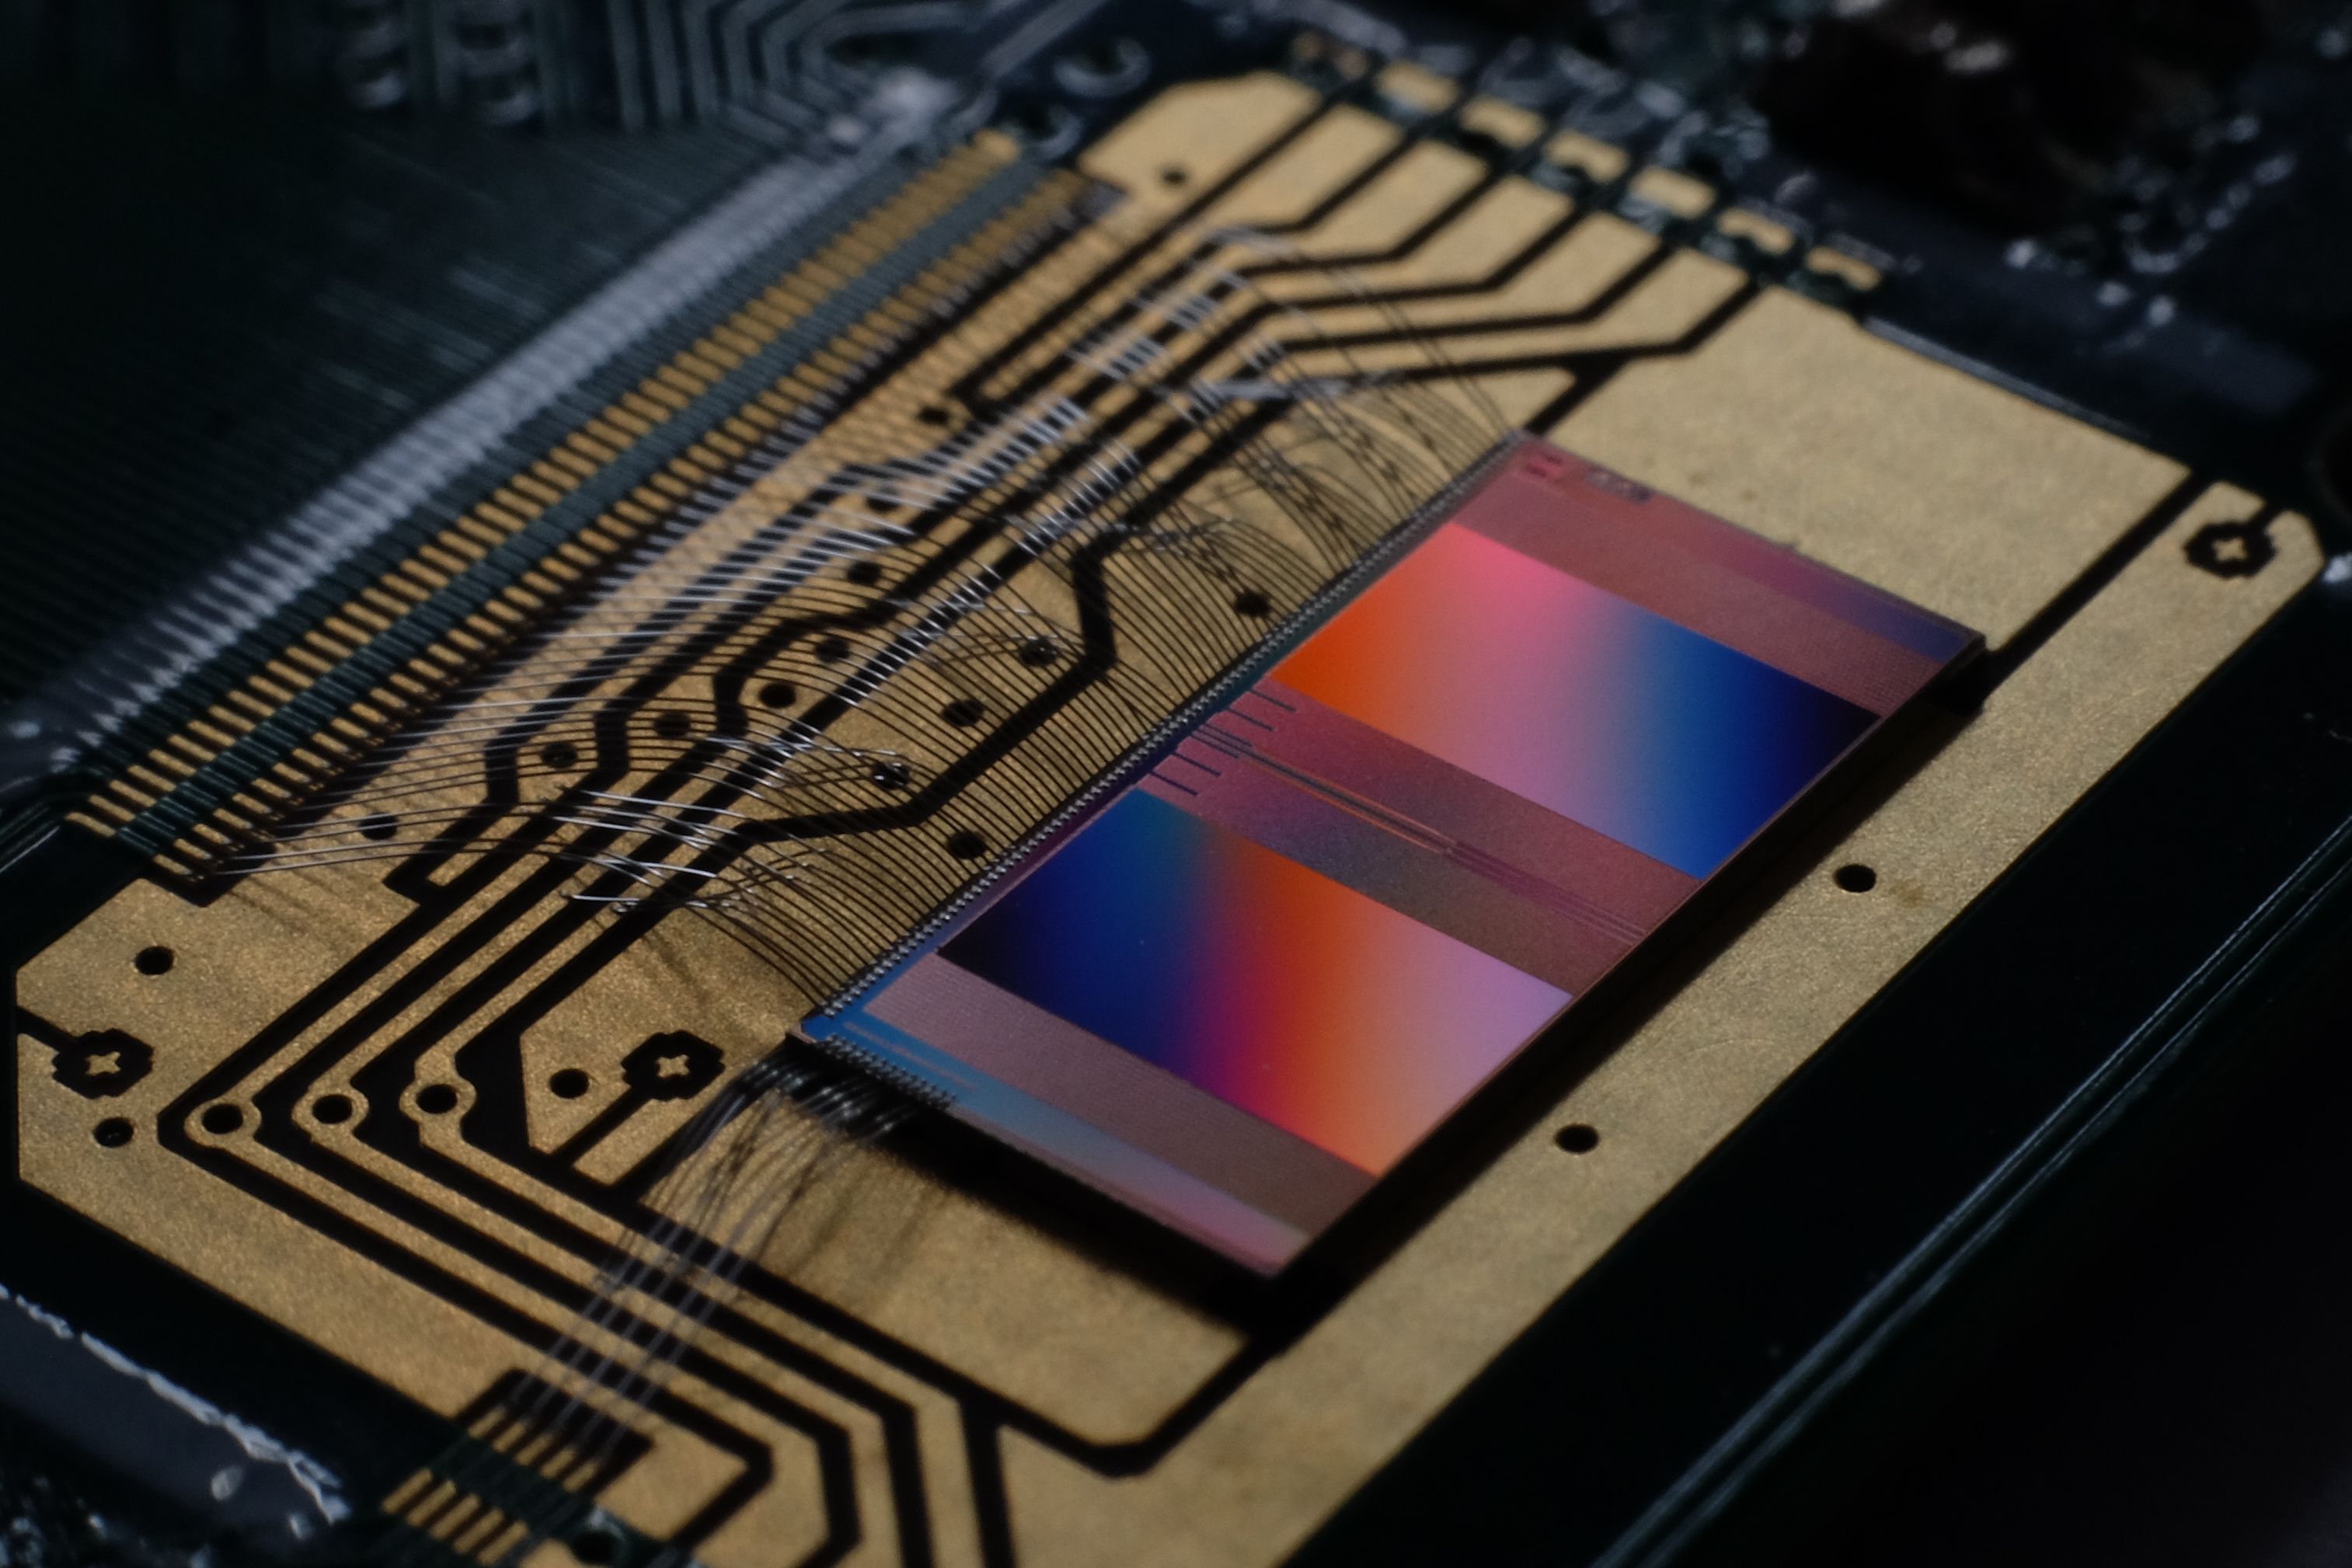
\includegraphics[width=.58\columnwidth]{images/chip.JPG}};
		\node[anchor=north west,inner sep=0pt] (a) at (0.1,0.0) {\tikzset{%
	inh/.style = {%
		draw=nicered,%
		fill=nicered,
		circle,
		inner sep=0pt,
		minimum width=0.3cm,
	},%
	exc/.style = {%
		draw=niceblue,%
		fill=niceblue,
		regular polygon,
		regular polygon sides=3,
		minimum width=0.4cm,
		inner sep=0pt,
	},%
}%
\pgfmathsetseed{42}%

\begin{tikzpicture}[
		x=2.3cm,
		y=2.3cm,
		>=stealth,
		line width=1.0\pgflinewidth,
		anchor=center
        ]

	\useasboundingbox (-1.4,0.65) rectangle (0.7,-0.82);

	% network layers
	\foreach \b in {0,1,...,4}{
		\ifthenelse{\b=3}{
			\node[inh] (background \b) at (-1.2,0.5-0.25*\b) {};
		}{
			\node[exc] (background \b) at (-1.2,0.5-0.25*\b) {};
		}
	}

	\pgfmathsetmacro{\N}{9}
	\pgfmathsetmacro{\r}{0.45}
	\coordinate (center) at (0,0);
	\foreach \n in {0,1,...,\N}{
		\ifthenelse{\n=2 \OR \n=5}{
			\node[inh] (hidden \n) at ($({\r*sin(\n*360/(\N+1))},{\r*cos(\n*360/(\N+1))})+(center)$) {};
		}{
			\node[exc] (hidden \n) at ($({\r*sin(\n*360/(\N+1))},{\r*cos(\n*360/(\N+1))})+(center)$) {};
		}
	}

        \begin{scope}[on background layer]
			% connectivity
			\begin{scope}
			\path[scope fading=south] (-0.8,-0.1) rectangle ++(1.6,-2.0);
			\foreach \h in {0,1,...,\N}{
				\foreach \i in {0,1,...,4}{
    	        			\pgfmathparse{rnd}
    	        			\pgfmathsetmacro{\foobar}{\pgfmathresult}
    	        			\ifthenelse{\lengthtest{\foobar pt<0.2 pt}}{
						\ifthenelse{\i=3}{
							\draw[-stealth,nicered] (background \i) -- (hidden \h);
						}{
							\draw[-stealth,niceblue] (background \i) -- (hidden \h);
						}
					}{}
				}
			}
			\end{scope}
			
			\fill[white,opacity=0.7] (0,0) circle (1.5cm);
			\draw[nicegray,semithick] (0,0) circle (1.5cm);

			\foreach \i in {0,1,...,\N}{
				\foreach \j in {0,1,...,\N}{
					\ifthenelse{\equal{\j}{0}}{
						% no self connections
					}{
						\pgfmathparse{rnd}
						\pgfmathsetmacro{\foobar}{\pgfmathresult}
						\ifthenelse{\lengthtest{\foobar pt<0.2 pt}}{
							\pgfmathsetmacro{\bend}{ifthenelse(\j <= \N / 2 + 1,"bend right","bend left"))}
							\pgfmathsetmacro{\target}{int(Mod(\i + \j, \N + 1))}
							\ifthenelse{\i=2 \OR \i=5}{
								\draw[-stealth,nicered] (hidden \i) to[\bend] (hidden \target);
							}{
								\draw[-stealth,niceblue] (hidden \i) to[\bend] (hidden \target);
							}
						}{}
				}
				}
			}
		\end{scope}

	\coordinate (label) at (0.0,-0.77);
	\node[nicegray,anchor=center] at (label -| hidden 0) {\footnotesize Network};
	\node[nicegray,anchor=center] at (label -| background 0) {\footnotesize Input};
\end{tikzpicture}
};
		\node[anchor=north west,inner sep=0pt] (c) at (5.15,0.0) {\input{build/figures/rate_evolution.pgf}};
		\node[anchor=north west,inner sep=0pt] (d) at (5.15,-3.8) {\input{build/figures/final_rate.pgf}};
		\node[anchor=north west,inner sep=0pt] (e) at (9.3,0.0) {\input{build/figures/weight_histogram.pgf}};
		\node[anchor=north west,inner sep=0pt] (f) at (9.3,-3.8) {\input{build/figures/connectivity.pgf}};
		\node[anchor=north west,inner sep=0pt] (g) at (13.45,-3.8) {\input{build/figures/average_weight.pgf}};
		\node at ($(a.north west) + (0.1,-0.2)$) {\textbf{A}};
		\node[text=white] at ($(b.north west) + (0.2,-0.2)$) {\textbf{B}};
		\node at ($(c.north west) + (0.2,-0.2)$) {\textbf{C}};
		\node at ($(d.north west) + (0.2,-0.2)$) {\textbf{D}};
		\node at ($(e.north west) + (0.2,-0.2)$) {\textbf{E}};
		\node at ($(f.north west) + (0.2,-0.2)$) {\textbf{F}};
		\node at ($(g.north west) + (0.2,-0.2)$) {\textbf{G}};
	\end{tikzpicture}

	\caption{%
		\textbf{Reducing the input strength to homeostatically regulated networks of \gls{ei} \gls{lif} neurons strengthens recurrent connections.}
		\textbf{(A)} Illustration of a random network topology with \SI{80}{\percent} excitatory (blue triangles) and \SI{20}{\percent} inhibitory (red circles) neurons.
		\textbf{(B)} Image of the BrainScaleS-2 neuromorphic chip.
		Image taken from \citep{muller_extending_2020}.
		\textbf{(C)} Homeostatic plasticity regulates the population rate $\nu$ close to a target value (dashed line).
		\textbf{(D)} For a broad range of external input rates, $\nu$ approximates the target rate.
		\textbf{(E)} The stochastic homeostatic regulation leads to heterogeneous weight distributions for both, inhibitory and excitatory synapses.
		The counts of excitatory weights exceed the inhibitory ones by a factor of four due to the imposed \gls{ei} ratio.
            \textbf{(F)} The effective connectivity, defined as the percentage of non-zero recurrent synapses ($c_{ij}w^\mathrm{rec}_{ij}\neq 0$), does not saturate at its maximum (dashed line) for decreasing input strengths.
		\textbf{(G)} However, the mean weight increases to compensate for a reduction of input.
	}
	\label{fig:chip}
\end{figure*}

\section{\label{sec:results}Results}

%\subsection{Reducing external input to homeostatically regulated neuromorphic hardware strengthens recurrent connections}
\subsection{Homeostatically regulated neuromorphic hardware compensates lack of external input by strengthening recurrent connections}

% homeostatic regulation
To begin, we verify that the experimental setup --- the neuromorphic chip with homeostatic regulation during development --- reaches a stationary dynamical state with firing rates sufficiently close to the target rate.
Starting from the initial condition of zero recurrent weights ($w^\mathrm{rec}_{ij}=0$), we observe for our chosen parameters a transient relaxation behavior that reaches a stationary firing rate after about \SI{200}{} update iterations, independent of the external input rate $h$ (\cref{fig:chip}C).
Note that for this representation, the firing rate is evaluated over an interval of $T=\SI{100}{\second}$ between iterations, and further averaged over \num{50} network realizations.
One can see that for larger values of $h$ (blue curve) the relaxation is smoother than for lower values of $h$ (red curve).
The stationary firing rates are close to the target rate $\nu^\ast=\SI{10}{\hertz}$ (\cref{fig:chip}D), however, there is a systematic $h$-dependence that presumably originates from the firing rate being a non-linear function of the mean coupling, $\nu(\langle w\rangle)$, as observed in mean-field calculations of \gls{ei} networks~\cite{mastrogiuseppe_intrinsically-generated_2017}. %which might in turn promote unstable activity further enhanced by the limited precision weight dynamics.
%Since, in this work, we do not seek a perfect match of the target rate but are interested in the self-organized collective dynamics of homeostatically regulated networks in general, we conclude that the homeostatic-plasticity rule reliably regulates the neuron firing rates sufficiently close to the target firing rate.
Since we find consistent results for reference computer simulations (see Supplemental Material), we conclude that the experimental setup reliably self-organizes into a stationary dynamics state with neuron firing rates sufficiently close to the target rate.

% reducing input strengthens recurrency
We next investigate how homeostatically regulated \gls{ei} networks compensate a reduction of external input with a strengthening of recurrent connections (\cref{fig:chip}E-G).
In particular, we find that the histograms of both inhibitory as well as excitatory recurrent coupling weights become flatter with decreasing $h$, indicating strong heterogeneity (\cref{fig:chip}E).
%It is noteworthy that the limited range of weight values is an effect of the \SI{6}{\bit} integer weights on the neuromorphic hardware.
Interestingly, the effective connectivity -- the fraction of all physical $K^\mathrm{rec}$ recurrent weights that are not zero -- does not reach its maximum theoretical value of $K^\mathrm{rec}/N = 100 / 512 \approx \SI{20}{\percent}$ (\cref{fig:chip}F).
Instead, it even decreases for low $h$, which is likely a consequence of the strong variability of rates between iterations (cf. \cref{fig:chip}C) that results in large weight changes for the given plasticity rule and does not affect our main conclusions (see Supplemental Material for a milder plasticity rule).
%This assumption is further strengthened by a reduced decline of the effective connectivity for a non stochastic and hence more continuous implementation of homeostatic regulation (\cref{fig:hom_comparison}B).

\begin{figure*}[ht]
	\centering
	\begin{tikzpicture}
		\node[anchor=north west,inner sep=0pt] (x) at (0.94,-3.8) {\import{build/figures/}{colorbar.pgf}};
		\node[anchor=north west,inner sep=0pt] (a) at (0,0) {\input{build/figures/ac.pgf}};
		\node[anchor=north west,inner sep=0pt] (b) at (4.2,0) {\input{build/figures/activity_distribution.pgf}};
		\node[anchor=north west,inner sep=0pt] (c) at (8.5,0) {\input{build/figures/activity.pgf}};
		\node[anchor=north west,inner sep=0pt] (d) at (13.6,0) {\input{build/figures/timescale_comparison.pgf}};
		\node at ($(a.north west) + (0.2,-0.2)$) {\textbf{A}};
		\node at ($(b.north west) + (0.2,-0.2)$) {\textbf{B}};
		\node at ($(c.north west) + (0.2,-0.2)$) {\textbf{C}};
		\node at ($(d.north west) + (0.2,-0.2)$) {\textbf{D}};

		\draw[-latex,ultra thick] ($(c.north east) + (0.2,-0.15)$) -- ($(c.south east) + (0.2,0.8)$) node[midway,xshift=0.2cm,rotate=-90] {Bistability};
	\end{tikzpicture}
	\caption{%
		\textbf{Reducing the input strength increases autocorrelation of network rate through emergent bistability.}
        \mbox{\textbf{(A)} For} low input rates $h$, the population activity exhibits exponentially shaped autocorrelations $C(t')$ with autocorrelation times $\tau_\mathrm{AC}$ significantly exceeding the largest single neuron timescale.
		\textbf{(B)} In this regime, the distribution $P(\nu)$ of the population rate $\nu$ shows a bimodal trend.
		\textbf{(C)} The associated phases of high and low $\nu$ can be fitted by a two state \acrshort{hmm}.
		\textbf{(D)} Based on the transition rates of this \acrshort{hmm}, an equivalent timescale $\tau_\mathrm{HM}$ can be estimated which coincides with $\tau_\mathrm{AC}$ for low $h$.
	}
	\label{fig:time_scale}
\end{figure*}

More important is the observation that, as shown in \cref{fig:chip}G, the mean coupling weights $w^\mathrm{rec}$ increase almost linearly with decreasing input rate.
%In addition to the observed heterogeneity, we clearly find that the mean inhibitory and excitatory weights increase almost linearly with reducing the input rate (\cref{fig:chip}G).
A fit of the form
\begin{equation}\label{eq:w-h}
    \langle w^\mathrm{rec}\rangle(h) = \alpha - \beta h,
\end{equation}
where $\langle.\rangle$ stands for average across synaptic connections over either excitatory or inhibitory populations, yields $\alpha\approx\SI{22.75}{}$ and $\beta\approx\SI{14.23}{}$ for excitatory or $\alpha\approx\SI{26.1}{}$ and $\beta\approx\SI{16.7}{}$ for inhibitory weights.
Hence, a reduction in input rate clearly strengthens the recurrent connections in homeostatically regulated \gls{ei} networks consistent with the theoretical consideration that the loss of external input needs to be compensated by recurrent activity generation in order to maintain a constant firing rate~\cite{zierenberg_homeostatic_2018}.



% E-I balance
In addition to supporting general theoretical arguments, our setup allows us to investigate how our homeostatic self-organization affects the interplay between excitatory and inhibitory neurons.
In fact, it is quite surprising that the mean coupling weights for excitatory and inhibitory weights are so similar (\cref{fig:chip}G), i.e., $\langle w^\mathrm{rec}_\mathrm{inh} \rangle \approx \langle w^\mathrm{rec}_\mathrm{exc}\rangle$, given that each neuron receives four times more input from excitatory than from inhibitory neurons.
Naively, this implies strong excitation dominance in contrast to the expected inhibition dominance required for asynchronous irregular activity~\cite{vreeswijk_chaos_1996,brunel_dynamics_2000} to reproduce experimental single-neuron statistics~\cite{burns_spontaneous_1976, softky_highly_1993, stevens_input_1998, stein_neuronal_2005}.
This outcome can, however, be explained by our symmetric plasticity rule that does not distinguish between excitatory and inhibitory synapses and thereby fosters solutions with $\langle w^\mathrm{rec}_\mathrm{inh} \rangle \approx \langle w^\mathrm{rec}_\mathrm{exc}\rangle$.
For small networks with homogeneous weights (see \cref{sec:phase_diagrams}), the condition $w^\mathrm{rec}_\mathrm{inh} \approx w^\mathrm{rec}_\mathrm{exc}$ turns out to be in the vicinity of a phase transition between regular (high-firing) and irregular (low-firing) dynamics.
Reducing $h$ makes this transition more abrupt and closer to $w^\mathrm{rec}_\mathrm{inh} = w^\mathrm{rec}_\mathrm{exc}$, implying that homeostatic plasticity regulates \gls{ei} networks towards a regular-to-irregular transition when decreasing the external input rate.

% now theoretical prediction of increasing autocorrelation time
\subsection{Homeostatically regulated neuromorphic hardware with low external input generates large autocorrelation times through emergent bistability}

Next, we verify the theoretical prediction~\cite{zierenberg_homeostatic_2018} that a homeostatically regulated system exhibits an increased autocorrelation to compensate for a decreasing external input (\cref{fig:time_scale}).
For this, we consider a network after homeostatic development with fixed weights and evaluate the autocorrelation function of the population firing rate $\nu(t)$ over an interval of $T=\SI{100}{\second}$.
Indeed, the autocorrelation functions, $C(t^\prime)$, show increasingly long tails with decreasing input rate $h$ (\cref{fig:time_scale}A).
Moreover, they are well described by exponential decays, $C(t^\prime)=e^{-t^\prime/\tau_\mathrm{AC}}$, with increasing autocorrelation times $\tau_\mathrm{AC}$ for decreasing $h$ (\cref{fig:time_scale}A inset).
While this general trend has been reported for much smaller neuromorphic systems before~\cite{cramer_control_2020}, the inset of Fig.~\ref{fig:time_scale}A reveals the emergence of two distinct regimes.
For $h>\SI{0.8}{\kilo\hertz}$, we find autocorrelation times to saturate with increasing $h$, suggesting that the uncorrelated Poisson input successfully decorrelates already weakly correlated activity, giving rise to an \textit{input-driven regime}.
In contrast, for $h<\SI{0.8}{\kilo\hertz}$, we find an apparent divergence of $\tau_\mathrm{AC}$ with decreasing $h$, such that this regime is characterized by dominant recurrent activation compensating for the lacking input, which results in increasing autocorrelation times for decreasing $h$, giving rise to a \textit{recurrent-driven regime}.

Surprisingly, we observe that the autocorrelations originate from a bistable population rate (\cref{fig:time_scale}B-D).
Specifically, the distribution $P(\nu)$ changes from unimodal for higher input strengths to bimodal for lower input strengths (\cref{fig:time_scale}B).
The latter suggests that the population rate starts to alternate between two distinct states.
Indeed, close inspection of the time evolution of $\nu(t)$ reveals that for decreasing input strength the population rate switches between a low-rate state and a high-rate state (\cref{fig:time_scale}C), resembling up-and-down states in cortical networks~\cite{wilson_up_2008,stern_spontaneous_1997,cossart_attractor_2003,hidalgo_stochastic_2012}.
Such a switching behavior is reminiscent of a Markov jump process between states of high- and low-firing rates~\cite{ibe_3_2013}, specifically a two-state \gls{hmm}~\cite{rabiner_introduction_1986}.
We fitted a two-state \gls{hmm} to the stationary population rate (discretized in steps of $\Delta t$) and obtained a $2\times 2$ Markov matrix.
%using the Python toolbox hmmlearn~\cite{noauthor_hmmlearnhmmlearn_2022}, which returns a $2\times 2$ Markov matrix for a stationary process.
Since the rate is stationary, the first eigenvalue is one, $\lambda_1=1$, and the second eigenvalue $\lambda_2$ determines how quickly perturbations decay back to the stationary solution.
This is related to the autocorrelation time as $\tau_\mathrm{HM}=-\Delta t/ \log{(\lambda_2)}$.
Indeed, the autocorrelation time of the \gls{hmm} correlates with the autocorrelation time measured from the population rate for small input strengths, where the population rate becomes bistable (\cref{fig:time_scale}D).
This is fundamentally different from the \textit{a-priori} expected close-to-critical fluctuations~\cite{zierenberg_homeostatic_2018}, which would lead to scale-free avalanches~\cite{beggs_neuronal_2003} for small $h$ that we do not observe (see \cref{sec:avalanches}).
We thus conclude that the emergent bistability is the underlying mechanism of the large autocorrelation times observed in the population dynamics of homeostatically regulated \gls{ei} networks of \gls{lif} neurons.






%Instead, the network dynamics are better described as a Markov jump process between states of high- and low-firing rates~\cite{ibe_3_2013}.
%The population rate can be well approximated by a two-state \gls{hmm}~\cite{rabiner_introduction_1986}.
%    We fitted a two-state \gls{hmm} to the population rate (discretized in steps of $\Delta t$) using Python toolbox hmmlearn~\cite{noauthor_hmmlearnhmmlearn_2022}, which returns a $2\times 2$ transition matrix.
%    \textcolor{blue}{TODO: WHY, what is the largest eigenvalue}
%The second-largest eigenvalue of this matrix, $\lambda_2$, is the autocorrelation time of Markov process, $\tau_\mathrm{HM}=-\Delta t/ \log{(\lambda_2)}$.
%Indeed, the autocorrelation time of the \gls{hmm} correlates with the autocorrelation time measured from the population rate for small input strengths, where the population rate becomes bistable (\cref{fig:time_scale}D).
%We thus conclude that the emergent bistability is the underlying mechanism of the large autocorrelation times observed in the population dynamics of homeostatically regulated \gls{ei} networks of \gls{lif} neurons.

\subsection{Computer simulations reveal increasing dynamical barrier of emergent bistability with system size}

Since our neuromorphic hardware only supports networks with up to $512$ \gls{lif} neurons, we use computer simulations to verify the experimental results for increasing network sizes.
In brief, we parametrize the simulations to match the experimental setup and use the Brian2 Python package to solve the model (for details see \cref{sec:methods}).
Indeed, we can reproduce the experimental results with our software implementation: We observe comparable bistable activity with similar autocorrelation functions (see Supplemental Material).
However, while computer simulations in principle allow us to study any system size, they are much less efficient than the neuromorphic emulation.
It is worth noting that for our application, i.e., homeostatically regulating a network of $N=512$ \gls{lif} neurons for \SI{6000}{\second}, the computer simulation on an Intel Xeon E5-2630v4 (roughly $\SI{100 000}{\second}$ at about $\SI{50}{\watt}$) takes $\mathcal{O}(10^4)$ more time and $\mathcal{O}(10^7)$ more energy compared to the corresponding emulation on BrainScaleS-2 (about $\SI{6}{\second}$ at a power budget of \SI{100}{\milli\watt}).


%While on BrainScaleS-2 the emulation of a network with $N=512$ \gls{lif} neurons for \SI{6000}{\second} including homeostatic regulation takes about $\SI{6}{\second}$ at a power budget of \SI{100}{\milli\watt}, a corresponding computer simulation on an Intel Xeon E5-2630v4 amounts to around $\SI{30}{\hour}$ at approximately \SI{50}{\watt}.
%This makes the emulation much faster and about $10^7$ times more energy efficient than the simulation.

\begin{figure}[t]
	\centering
	\begin{tikzpicture}
		\node[anchor=north west,inner sep=0pt] (a) at (0,0) {\input{build/figures/simulation_ac.pgf}};
		\node[anchor=north west,inner sep=0pt] (b) at (4.2,0) {\input{build/figures/simulation_activity_distribution.pgf}};
		\node at ($(a.north west) + (0.2,-0.2)$) {\textbf{A}};
		\node at ($(b.north west) + (0.2,-0.2)$) {\textbf{B}};
	\end{tikzpicture}
	\caption{%
		\textbf{Finite-size scaling of homeostatically regulated \gls{ei} networks with \gls{lif} neurons from computer simulations.}
		\textbf{(A)} Autocorrelation time $\tau_\mathrm{AC}$ as a function of system size $N$ for different external input rates $h$.
        One can see a faster than power-law growth for $h<\SI{0.8}{\kilo\hertz}$, while $\tau_\mathrm{AC}$ seems to saturate on the order of the dominant single-neuron timescale (dashed line) for $h>\SI{0.8}{\kilo\hertz}$.
		\textbf{(B)} Distributions of the population firing rate in windows of $\SI{5}{\milli\second}$ for $h=\SI{0.7}{\kilo\hertz}$ show the bimodal shape remains for increasing $N$.
		The barrier in between high- and low-firing states grows with $N$.
    	}
	\label{fig:sim}
\end{figure}

Having established that the computer simulation reproduces the experimental results, we can study how the measured autocorrelation time $\tau_\mathrm{AC}$ depends on the network size $N$ (\cref{fig:sim}A).
Due to the large computational efforts, we focus on four representative input strengths: a low input strength ($h=\SI{0.7}{\kilo\hertz}$) where we observe bistable activity in the experiment, two medium input strengths ($h=\SI{0.8}{\kilo\hertz}$ and $h=\SI{0.9}{\kilo\hertz}$) near the onset of bistability, and a high input strength ($h=\SI{1.0}{\kilo\hertz}$) where the network does not exhibit bistability.
Only for $h=\SI{0.7}{\kilo\hertz}$, we observe an exponential increase in autocorrelation time with system size that exceeds $\SI{1}{s}$ for the largest $N$.
Instead, at $h=\SI{0.8}{\kilo\hertz}$ the autocorrelation time appears to grow as a power law, while for even larger values of $h$ the $\tau_\mathrm{AC}$ start to saturate on the order of the dominant single-neuron timescale (dashed line).
Our numerical results further corroborate the classification into two distinct regimes: A recurrent-driven regime for low input strength with large emergent autocorrelations and the input-driven regime for high input strength with vanishing autocorrelations.
%The transition between these regimes can be studied in a more systematic way employing finite-size scaling analyses.

To further investigate the origin of the emergent autocorrelations, we study the shape of the probability distribution of local population rates $\nu(t)$ as a function of network size (\cref{fig:sim}B).
We observe that for low input strength, the bimodal distribution becomes more pronounced with increasing suppression of intermediate population-rate values.
%TODO: What is with the other two cases...SI!!! but plot
One can relate the suppression of intermediate rates to a \textit{dynamical barrier} by interpreting the time course of the instantaneous population rates as a trajectory of the dynamical system in the potential $V(\nu) = -\log P(\nu)$.
This barrier would be analogous to the activation energy in an Arrhenius-type equation, i.e., $r\propto e^{-\Delta V/T}$, such that for a given level of fluctuation $T$ the rate $r$ to transition between low- and high-firing-rate regimes is lowered for increasing barriers $\Delta V$.
Since the height of this dynamical barrier increases with $N$, this explains the increasing autocorrelation time with system size.


\begin{figure}[t]
	\begin{tikzpicture}
		\node[anchor=north west,inner sep=0pt] (a) at (0,0)  {\input{build/figures/theory_potential.pgf}};
		\node[anchor=north west,inner sep=0pt] (b) at (4.2,0){\input{build/figures/theory_activity.pgf}};
		\node at ($(a.north west) + (0.2,-0.2)$) {\textbf{A}};
		\node at ($(b.north west) + (0.2,-0.2)$) {\textbf{B}};
	\end{tikzpicture}
	\caption{%
        \textbf{Mean-field theory of emergent bistability upon reducing input to homeostatically regulated recurrent network.}
        Our mean-field theory describes the temporal evolution of the fraction of active neurons, $\rho$, with meta-stable solutions given by the minimum of the potential, \cref{eq:potential}.
        \textbf{(A)} For suitable parameters ($\tau_\mathrm{MF}=10$, $\alpha=30$, $\beta=15$, $b=25$, $\sigma=50$, $N=512$), the potential exhibits a single minimum for large $h$ but two minima for small $h$.
        \textbf{(B)} Numeric evaluation of the corresponding stochastic mean-field equation ($\Delta t=10^{-7}$) shows fluctuating dynamics for large $h$ and emergent bistability for low $h$.
        }
	\label{fig:theory}
\end{figure}



\subsection{Mean-field theory of emergent bistability from fluctuation-induced switching between metastable active and quiescent states}

To qualitatively explain how bistability can emerge in recurrent network with heterogeneous weights, we construct a simple mean-field theory based on the time evolution of a fraction of active neurons at a given time $t$, $\rho(t)$, which can be considered a proxy of the population rate $\nu(t)$ up to some factor.
Let us consider a general mean-field ansatz
\begin{align}
	\dot{\rho}(t) = &-\tau_\mathrm{MF}\rho(t) \nonumber \\
		&+h  (1-\rho(t)) + \left( 1-\rho(t) \right) \left[ \omega_1\rho(t) + \omega_2\rho^2(t)+\dots\right]\, ,
\end{align}
%
where the first term describes the spontaneous decay of activity in the absence of inputs with some characteristic time scale
$\tau_\mathrm{MF}$, the term proportional to $h$ represents external input that can only activate inactive neurons (hence the $(1-\rho)$ factor), and the last term represent the gain function that describes recurrent activations, expanded in power-series of the activity.
Here, the coefficients of expansion ($\omega_1$, $\omega_2$, ...) are an effective representation of the full coupling matrix $w^\mathrm{rec}_{ij}$ (with $\omega_1$ proportional to the mean synaptic strength).
The mean-field equation can be rewritten in a more compact form by grouping-up terms with different powers of the activity,
\begin{equation}\label{eq:MF_compact}
    \dot{\rho}(t) = h - a\rho(t) -b\rho^2(t) + \dots \, ,
\end{equation}
%
where $a=\tau_\mathrm{MF}+h-\omega_1$ and $b=\omega_1-\omega_2>0$ to ensure stability.
It is important to notice that this mean-field equation assumes infinitely large network sizes, $N\to\infty$, for which additional noise terms vanish.

%finite
To describe finite networks one needs to introduce an additional stochastic term to the mean-field \cref{eq:MF_compact} that accounts for demographic fluctuations.
Demographic fluctuations are characteristic of systems with an absorbing or quiescent state~\cite{henkel_absorbing_2008}, where fluctuations of the total number of active units around some mean $N\rho(t)$ are expected to have a standard deviation that scales with $\sqrt{N\rho(t)}$ as a consequence of the central-limit theorem.
For the fraction of active nodes in a finite network, we then obtain to leading order in system size
\begin{equation}\label{eq:MF_noise}
    \dot{\rho}(t) = h - a\rho(t) -b\rho^2(t) + \sqrt{\rho(t)/N}\eta(t)\, ,
\end{equation}
where $\eta(t)$ is Gaussian white noise with zero mean and variance $\sigma^2$.
This (Ito) Langevin equation can be expressed as a Fokker Planck equation, with the steady-state solution~\cite{munoz_nature_1998} (see also SI)
\begin{equation}
    P(\rho) = \mathcal{N}\exp\left\{-\frac{2N}{\sigma^2}V(\rho)\right\}\, ,
\end{equation}
a normalization constant $\mathcal{N}$, and the potential
\begin{align}\label{eq:potential}
    V(\rho) = \left(\frac{\sigma^2}{2N} - h\right)\ln\rho + a\rho + \frac{b}{2}\rho^2\, .
\end{align}
This potential $V(\rho)$ can either have a single (formally diverging) minimum at $\rho=0$ (unimodal activity distribution), or it can have two local minima (bistable activity distribution).
%Specifically, we can find from the condition $\rho\,dV/d\rho=(\frac{\sigma^2}{2N}-h) + a\rho +b\rho^2=0$ extrema at $\rho_\pm = \left(-a\pm\sqrt{a^2-4b(\frac{\sigma^2}{2N}-h)}\right)/2b$ such that a bistable solution occurs when
The condition for extrema of the potential $V$ imply that a bistable solution occurs when
%\begin{equation}\label{eq:condition-bistable}
    $a^2-4b(\frac{\sigma^2}{2N}-h)>0$.
%\end{equation}
With the additional conditions for a positive density, i.e., $\rho>0$, as well as a positive slope at $\rho=0$, i.e., $\rho^2\frac{d^2V}{d\rho^2}(0)=(\frac{\sigma^2}{2N}-h)>0$, we expect to observe bistable dynamics for
\begin{equation}\label{eq:condition-bistable}
    a<-2\sqrt{b\left(\frac{\sigma^2}{2N}-h\right)}<0.
\end{equation}

% homeostatic regulation
To incorporate the effect of training recurrent weights with homeostatic regulation, we recall our empirically obtained anticorrelation, $\langle w \rangle = \alpha - \beta h$, upon homeostatic training (\cref{fig:chip}G).
In our mean-field theory, \cref{eq:MF_compact}, we assume this to dominantly affect $a=\tau_\mathrm{MF} + h - \omega_1 \approx \tau_\mathrm{MF}  - \alpha + h(1+\beta)$ and make the common assumption that $b=\omega_1-\omega_2$ is constant up to higher-order effects.
Inserting $a$ into \cref{eq:condition-bistable}, we find that ---for suitable parameters--- lowering $h$ can indeed induce a transition from a unimodal to a bimodal potential (\cref{fig:theory}).
%Then the condition for a bistable solution, \cref{eq:condition-bistable}, becomes $\tau_\mathrm{MF}-\alpha +h(1+\beta) < -2\sqrt{b(\frac{\sigma^2}{2N}-h)}$ and we find that ---for suitable parameters--- lowering $h$ does indeed induce a transition from a unimodal to a bimodal potential (\cref{fig:theory}).

% stochastic simulations
The $h$-dependent transition from unimodal to bimodal can be visualized by numerically evaluating the mean-filed model (\cref{fig:theory}B).
The numerical integration of \cref{eq:MF_noise} is straightforward~\cite{dornic_integration_2005}, but needs special care to avoid running into the domain of negative numbers due to numerical imprecisions (see Appendix~\ref{sec:appendix_meanfield}).
The resulting trajectories show typical demographic fluctuations for higher inputs and bistable activity for lower input.
Since the involved parameters are not easily related in an explicit way to the experiment, this theoretical result is a qualitative explanation of the observed effect and all parameters are in arbitrary units.

Our mean-field theory implies that emergent bistable population activity can be rationalized as a fluctuation-induced switching between a metastable active and a quiescent phase.
For a system with an absorbing to active non-equilibrium phase transition for vanishing input, we find that finite-size fluctuations are responsible for a metastable active state (high rate) and external fluctuations lead to a metastable quiescent state (low rate).
To transit from one state to another, the system needs to overcome a dynamical barrier, where the transition from high-to-low rate requires demographic noise, whereas the transition from low-to-high rate requires external noise.

\section{\label{sec:discussion}Discussion}

% summary: autocorrelations from bistability
In summary, we showed that networks of \gls{ei} \gls{lif} neurons with homeostatic regulation during training can self-organize for low external input into a dynamical regime with stochastic switching between states of high population firing rate (up state) and states of low population firing rate (down state).
Stochastic switching is the result of an emergent bistability, where a dynamical barrier between two metastable states (up and down) can be crossed due to fluctuations: finite-size activity fluctuations to cross up-to-down and external-noise fluctuations to cross down-to-up.
The crossing rate decreases with the barrier height, similar to classical nucleation rates decreasing for a larger free-energy barrier~\cite{feder_homogeneous_1966, kashchiev_nucleation_2000, zierenberg_canonical_2017}, and we showed numerically that the barrier height increases with system size.
Finally, a reduced crossing rate implies an increased autocorrelation time, which we demonstrated for both neuromorphic hardware and numerical simulations.
Our findings of large emergent autocorrelation times in networks of spiking neurons complements recent observations in networks regulated by spike-timing-dependent plasticity~\cite{cramer_control_2020} or when trained to perform working memory tasks~\cite{kim_strong_2021}.


Importantly, the stochastically-switching population activity that we observe does not require an active adaptation mechanism:
The emergent bistability was recorded in the testing phase after turning off homeostatic plasticity.
While plasticity was necessary to shape the weight distribution, it is not relevant for the stochastic switching between metastable-active (high rate) and metastable-absorbing (low-rate) states.
Our basic mechanism of a dynamical barrier that separates two metastable fixed points is consistent with previous observations of perturbation-induced state switching in spiking neural networks~\cite{brunel_effects_2001, renart_mean-driven_2006, tartaglia_bistability_2017}.
Here, we do not require additional, strong external perturbations, because we can control the height of the dynamical barrier and thereby observe the state switching induced by the available, weak external input during finite-time recordings.
%Importantly, the fluctuation-induced bistability is different from adaptation-based mechanisms, such as adaptation currents~\cite{parga_network_2007-1}, depletion of synaptic utility~\cite{millman_self-organized_2010} or self-organized bistability~\cite{di_santo_self-organized_2016, buendia_self-organized_2020}.
Importantly, the stochastic switching observed here is different from adaptation-based mechanisms, such as adaptation currents~\cite{parga_network_2007}, or depletion of synaptic utility~\cite{millman_self-organized_2010, bonachela_self-organization_2010}.

It is interesting to discuss more in depth the connection with the mechanism of self-organized bistability (SOB)~\cite{di_santo_self-organized_2016, buendia_feedback_2020} which has recently shown to be relevant for collective brain dynamics \cite{buendia_self-organized_2020}.
This is a mechanism akin to self-organized criticality (SOC)~\cite{bak_self-organized_1988, buendia_feedback_2020}, where the system self-organizes by means of a feedback-loop between the level of activity (overall firing rate) and the control parameter (the mean synaptic weight) to the edge of a phase transition.
In the case of SOB this is a discontinuous phase transition.
In the present case, there is a similar feedback loop during training.
But rather than acting on a global control parameter, this feedback acts differentially for each synaptic weight, thereby generating a broad weight distribution, which, for low external input, tunes the system to a bistable state at the edge of the transition between high and low firing rates.
Due to this bistability, in combination with external drive and finite-size fluctuations, we observe stochastic switching in the test phase (no homeostatic plasticity).

%The here identified mechanism of a stochastic state switching thereby presents a new perspective on so-called up-and-down states.
%Up-and-down states are defined on the level of a single-neuron membrane potential that switches between states with higher membrane potential resulting in spiking responses and those with lower membrane potential~\cite{wilson_up_2008}.
%While some of the aforementioned models utilize adaptation mechanisms to generate up-and-down states~\cite{millman_self-organized_2010,di_santo_self-organized_2016, buendia_self-organized_2020}, we here develop an alternative explanation:
%If neurons homeostatically regulate their firing rates, a decreasing external input can result in emergent autocorrelations with potential functional benefits~\cite{zierenberg_homeostatic_2018, cramer_control_2020} until a point where bistability can emerge on the population level.
%As a result of such (local) collective bistability, single neurons could switch between states of high and low synaptic input, which could in turn cause up-and-down states on the level of their membrane potentials.
%Such up-and-down states have been demonstrated as a collective effect of pathological bursts in neuronal cultures~\cite{vardi_simultaneous_2016}, but also more subtle in striatal~\cite{wilson_up_2008,stern_spontaneous_1997} and cortical~\cite{cossart_attractor_2003} areas.
%Our results provide new paths to test whether such observations of up-and-down states are connected to emergent bistability from homeostatic regulation via in-vitro assays or experiments with sensory deprivation.

The here identified mechanism of a stochastic state switching thereby presents a new perspective on so-called up-and-down states.
Up-and-down states are defined on the level of a single-neuron membrane potential that switches between states with higher membrane potential, resulting in spiking responses, and those with lower membrane potential~\cite{wilson_up_2008}.
While some of the aforementioned models utilize adaptation mechanisms to generate up-and-down states~\cite{millman_self-organized_2010,di_santo_self-organized_2016, buendia_self-organized_2020}, we here develop an alternative explanation:
If neurons homeostatically regulate their firing rates, a decreasing external input can result in emergent autocorrelations with potential functional benefits~\cite{zierenberg_homeostatic_2018, cramer_control_2020} until a point where bistability can emerge on the population level.
As a result of such emergent bistability, single neurons would switch between states of high and low synaptic input, which could in turn cause up-and-down states on the level of their membrane potentials.
This explanation is consistent with experimental observations of up-and-down states in striatal neurons~\cite{wilson_up_2008,stern_spontaneous_1997}, which focused on single-cell bistability, and in cortical slices~\cite{cossart_attractor_2003} and neuronal cultures~\cite{vardi_simultaneous_2016}, where up-and-down states were argued to be a collective (network) effect, and agrees with observations of bistability in networks of \gls{lif} neurons trained to store spatio-temporal patterns~\cite{scarpetta_hysteresis_2018}.
%, while our mean-field theory implies that the key mechanism is a stochastic switching that does not require a discontinous (``first-order'') non-equilibrium phase transition.
Our results thereby provide new paths to test whether experimental observations of up-and-down states are connected to emergent bistability from homeostatic regulation.


%Our general mean-field theory of fluctuation-induced bistability further presents a new paradigm for arbitrary finite systems with absorbing states and external drive.
%Examples of such systems include collective dynamics in epidemic spread~\cite{pastor-satorras_epidemic_2015} and ecosystems~\cite{scheffer_critical_2009, martin_eluding_2015}, catalytic reactions on surfaces~\cite{ehsasi_steady_1989}, calcium dynamics in living cells~\cite{bar_discrete_2000}, or turbulent liquid crystals~\cite{takeuchi_directed_2007,takeuchi_experimental_2009}.
%Indeed, for some of these systems the phenomenon of bistability has been observed, e.g., as switching behavior in disease models~\cite{bottcher_critical_2017}, for cellular automata with long-range interactions~\cite{pizzi_bistability_2021}, for CO oxidation~\cite{ertl_oscillatory_1991, suchorski_role_2018, wang_bistability_2019}, or as phase separation in active matter~\cite{martin_fluctuation-induced_2021,di_carlo_evidence_2022}.
%With our work, we present fluctuation-induced bistability as a new paradigm that should be observable (or avoidable) if the finite-size fluctuations are controlled accordingly.
Our simple mean-field theory implies that fluctuation-induced stochastic switching could be a very general effect in driven, finite systems with absorbing states.
Examples of such systems include collective dynamics in epidemic spread~\cite{pastor-satorras_epidemic_2015}, neural networks~\cite{beggs_neuronal_2003, chialvo_emergent_2010, wilting_25_2019}, ecosystems~\cite{scheffer_critical_2009, martin_eluding_2015}, and ultracold Rydberg atomic gases~\cite{helmrich_signatures_2020}, catalytic reactions on surfaces~\cite{ehsasi_steady_1989}, calcium dynamics in living cells~\cite{bar_discrete_2000}, or turbulence in liquid crystals~\cite{takeuchi_directed_2007, takeuchi_experimental_2009} and active nematics~\cite{doostmohammadi_onset_2017}.
Indeed, for some of these systems stochastic switching has been observed, e.g., as switching behavior in disease models~\cite{bottcher_critical_2017} or rate models of neural activity~\cite{van_meegen_large-deviation_2021}, for cellular automata with long-range interactions~\cite{pizzi_bistability_2021}, for CO oxidation~\cite{ertl_oscillatory_1991, suchorski_role_2018, wang_bistability_2019}, or as phase separation in active matter~\cite{martin_fluctuation-induced_2021, di_carlo_evidence_2022}.
Future work could include generalizing our results to systems that can be described by scalar fields, which is a common situation in non-equilibrium statistical physics, and investigate under what conditions one can observe (or avoid) stochastic switching on a macroscopic scale.



%We have shown a first demonstration how to exploit emergent autocorrelations due to bistability in spiking neural networks to encode information about an input even after stimulus offset.
%Reliable discrimination of the input rate was possible through the mean response across an ensemble of modules.
%While we here focused on discriminating the first moment of the input signal from a mean response, analogous to established concepts to quantify information processing capacities via a dynamic range~\cite{munoz_colloquium_2018, kinouchi_optimal_2006}, we expect that complex input statistics can be captured with tailored individual modules~\citep{zierenberg_tailored_2020} and that higher moments can be captured from higher-dimensional representations of the ensemble response through neural manifolds~\cite{gallego_neural_2017, gao_theory_2017}.
%These first results may serve as a foundation for a bottom-up approach towards a mechanistic understanding of information processing and towards practical applications of neuromorphic hardware that may exploit multi-chip architectures.


\section*{Acknowledgments}

This work has received funding from the European Union Sixth Framework Programme ([FP6/2002-2006]) under grant agreement no 15879 (FACETS), the European Union Seventh Framework Programme ([FP7/2007-2013]) under grant agreement no 604102 (HBP), 269921 (BrainScaleS) and 243914 (Brain-i-Nets) and the Horizon 2020 Framework Programme ([H2020/2014-2020]) under grant agreement no 720270, 785907, and 945539 (HBP), the Deutsche Forschungsgemeinschaft (DFG, German Research Foundation) under Germany’s Excellence Strategy EXC 2181/1-390900948 (the Heidelberg STRUCTURES Excellence Cluster), the Helmholtz Association Initiative and Networking Fund [Advanced Computing Architectures (ACA)] under Project SO-092 as well as the Manfred St\"{a}rk Foundation.
MAM acknowledges the Spanish Ministry and Agencia Estatal de investigaci{\'o}n (AEI) through Project of I+D+i Ref. PID2020-113681GB-I00, financed by MICIN/AEI/10.13039/501100011033 and FEDER “A way to make Europe”, as well as the Consejer{\'\i}a de Conocimiento, Investigaci{\'o}n Universidad, Junta de Andaluc{\'\i}a and European Regional Development Fund, Project P20-00173 for financial support.
VP and JZ were supported by the Max Planck Society.
JZ received financial support from the Joachim Herz Stiftung and the Plan Propio de Investigaci\'on y Transferencia de la Universidad de Granada.
The authors acknowledge support by the state of Baden-W\"{u}rttemberg through bwHPC.


\appendix
\begin{figure}[t]
	\centering
	\definecolor{blue}{HTML}{1f77b4}%
\definecolor{red}{HTML}{d62728}%
\definecolor{green}{HTML}{2ca02c}%
\definecolor{yellow}{HTML}{fee23e}%
\definecolor{hidden}{HTML}{005b82}%
\definecolor{input}{HTML}{af5a50}%
\definecolor{ppu}{HTML}{7d966e}%
\definecolor{output}{HTML}{555555}%
\tikzset{silent/.style={cross out, draw, 
         minimum size=2*(3pt-\pgflinewidth), 
	 inner sep=0pt, outer sep=0pt, thick}}
\tikzset{input_synapse/.style={circle,minimum size=0.17cm,inner sep=0pt,fill=input}}%
\tikzset{recurrent0_synapse/.style={circle,minimum size=0.17cm,inner sep=0pt,fill=hidden}}%
\tikzset{recurrent1_synapse/.style={circle,minimum size=0.17cm,inner sep=0pt,fill=output}}%
\pgfmathdeclarerandomlist{MyRandomSynapses}{%
    {input_synapse}%
    {recurrent0_synapse}%
    {recurrent1_synapse}%
    {silent}%
}%
\tikzset{block/.style={font={\rmfamily\footnotesize},align=center}}%
\tikzset{box/.style={draw=black!90}}%
\tikzset{block label/.style={fill=white,font={\rmfamily\footnotesize},inner sep=0.05cm}}%
\tikzset{%
	neuron/.style = {%
		draw=black,%
		circle,%
		inner sep=0pt,%
		minimum width=0.3cm%
	},%
	driver/.style = {%
		minimum height=0.7cm,%
		draw=black,%
		regular polygon,%
		regular polygon sides=3,%
		shape border rotate=-90,%
		inner sep=0pt%
	},%
}%
%
\begin{tikzpicture}[
		x=1.7cm,
		y=1.7cm,
	    	anchor=center,
        ]
        \pgfdeclarelayer{background layer}
        \pgfsetlayers{background layer,main}
        % \draw[use as bounding box,inner sep=0pt,draw=none] (-0.1,0.0) rectangle ++(5.5,4.5);

	\begin{scope}
		\foreach \x in {0,1,...,7} {
			\pgfmathparse{100*(\x>3)}
			\colorlet{currentcolor}{output!\pgfmathresult!hidden}
			
			\node[neuron,currentcolor,thick,inner sep=1pt] (nrn \x) at (0.8 + \x*0.5,0.35) {\fontsize{8}{8}\selectfont $t_\x^k$};
			\draw[stealth-] (nrn \x.north) ++ (0.0,0.01) -- ++(0.0,1.85);
		}

		\foreach \y [evaluate=\y as \z using {int(\y + 4)}] in {0,1,...,3} {
			\node[driver,thick] (drv \y) at ($(nrn 0) + (-0.5,0.5 + \y*0.5)$) {};
			\draw (drv \y.east) -- ++(3.8,0.0);
			\draw[stealth-,input,thick] ($(drv \y.center) + (-0.11,0.10)$) -- ++(-0.25,0.0) node[anchor=east] {\fontsize{8}{8}\selectfont $s_\y^l$};

			\foreach \x in {0,1,...,7} {
				\pgfmathrandomitem{\RandomSynapse}{MyRandomSynapses}
				\draw (drv \y -| nrn \x) node[\RandomSynapse] {};
			}
		}

		% routing
		\foreach \x in {0,1,2,3} {
			\draw[hidden,thick] (nrn \x.south) -- ++(0.0,-0.1) coordinate (tmp) -- (tmp -| drv 0.west) -- ++(-0.14,0.0) coordinate (sammelpunkt);
		}
		
		\foreach \y in {0,1,...,3} {
			\draw[-stealth,hidden,thick] (sammelpunkt) -- ($(sammelpunkt |- drv \y) + (0.0,0.00)$) coordinate (tmp) -- (tmp -| drv \y.west);
		}
		
		\foreach \x in {4,5,6,7} {
			\draw[output,thick] (nrn \x.south) -- ++(0.0,-0.16) coordinate (tmp) -- (tmp -| drv 0.west) -- ++(-0.2,0.0) coordinate (sammelpunkt);
		}
		
		\foreach \y in {0,1,...,3} {
			\draw[-stealth,output,thick] (sammelpunkt) coordinate (tmp) -- ($(tmp |- drv \y) - (0.0,0.1)$) coordinate (tmp) -- (tmp -| drv \y.west);
		}

		% ppu
		\node[rectangle,thick,draw,ppu,rounded corners,inner sep=2pt,minimum width=6.5cm] (ppu) at ($(nrn 0) + (1.9,2.7)$) {\fontsize{8}{8}\selectfont PPU};
		\foreach \x in {0,1,...,7} {
			\draw[ppu,-stealth] (nrn \x.55) -- ++(55:0.12) coordinate (tmp) -- (tmp |- ppu.south) node[pos=0.85, fill=white, inner sep=1] {\fontsize{8}{8}\selectfont $\nu_\x$};
		}
	\end{scope}
\end{tikzpicture}

	\caption{%
		\textbf{The connectivity on BrainScaleS-2 is physically represented by two arrays of synapses.}
		The routing capabilities of BrainScaleS-2 are utilized such that both arrays can be treated as a larger virtual one.
		Input events $s_i^l$ enter this array together with recurrent events $t_i^k$ (blue and gray) from the left via synapse drivers (triangles).
		The latter forward the events to a whole row of synapses (circles).
		Each synapse locally filters incoming events and either transmits input events (red) or recurrent events (blue and gray) to its home neuron.
		Sparsity is implemented by silencing out synapses (black crosses).
		Homeostatic regulation is carried on by the on-chip \acrshort{ppu} by accessing neuronal firing rates $\nu_i$ to update synaptic weights in a row-wise parallel manner.
	}
	\label{fig:routing}
\end{figure}

\section{Hardware details} \label{sec:appendix_hardware}

The connectivity on BrainScaleS-2 is physically represented by two arrays of synapses, each with a set of $256\times 256$ synapses.
Input spikes $s_i^l$ enter these arrays from the left via synapse drivers and are forwarded to a whole row of synapses.
Each synapse within this row locally filters incoming events, weights them according to a \SI{6}{\bit} weight and eventually transmits them to its home neuron.
The neurons are arranged in an additional row below the array of synapses.
Emitted neuronal spikes are injected back into the array via a flexible on-chip spike router.

Within this work, we exploit the routing capabilities of the BrainScaleS-2 system to unify both synapse arrays to a virtual array of size $256\times 512$ (\cref{fig:routing}).
The event filtering within each synapse located between synapse driver $i$ and neuron $j$ is used to either transmit the input events of spike source $i$ or the recurrent events of the neuron $i$ or $i + 256$, respectively.
We map our networks by configuring a random set of on average $K^\mathrm{rec}$ synapses per column of synapses to transmit recurrent events.
In addition, on average $K^\mathrm{in}$ randomly chosen synapses relay the input spike trains.
All remaining synapses are configured to transmit no events.

On BrainScaleS-2, the effect of each synapse, i.\,e.\, excitatory or inhibitory, is determined by the synapse drivers and is therefore a row-wise property within the synapse array.
For our networks, we program \SI{20}{\percent} of the synapse drivers (randomly selected) to be inhibitory.

The homeostatic plasticity is implemented on-chip by drawing on both \glspl{ppu} \citep{friedmann_demonstrating_2017}.
To that end, the number of emitted spikes is accessed and loaded into the \gls{simd} vector units of the \glspl{ppu} for subsequent weight update calculations.
Each vector unit allows to update a half-row of synaptic weights ($128$) synapses in parallel.
Calculations are performed with a precision of \SI{8}{\bit} in a fractional-saturation arithmetic.
The random numbers required to implement stochastic weight updates are directly drawn in parallel on-chip via dedicated accelerators.

\begin{figure*}[ht]
	\centering
	\begin{tikzpicture}
		\node[anchor=north west,inner sep=0pt] (a) at (0,0) {\input{build/figures/v_leak.pgf}};
		\node[anchor=north west,inner sep=0pt] (b) at (0,-3.6) {\input{build/figures/v_thres.pgf}};
		\node[anchor=north west,inner sep=0pt] (c) at (4.4,0) {\input{build/figures/v_reset.pgf}};
		\node[anchor=north west,inner sep=0pt] (d) at (4.4,-3.6) {\input{build/figures/tau_m.pgf}};
		\node[anchor=north west,inner sep=0pt] (e) at (8.8,0) {\input{build/figures/tau_syn_exc.pgf}};
		\node[anchor=north west,inner sep=0pt] (f) at (8.8,-3.6) {\input{build/figures/tau_syn_inh.pgf}};
		\node[anchor=north west,inner sep=0pt] (g) at (13.2,0) {\input{build/figures/epsp_height.pgf}};
		\node[anchor=north west,inner sep=0pt] (h) at (13.2,-3.6) {\input{build/figures/ipsp_height.pgf}};
		\node at ($(a.north west) + (0.2,-0.2)$) {\textbf{A}};
		\node at ($(b.north west) + (0.2,-0.2)$) {\textbf{B}};
		\node at ($(c.north west) + (0.2,-0.2)$) {\textbf{C}};
		\node at ($(d.north west) + (0.2,-0.2)$) {\textbf{D}};
		\node at ($(e.north west) + (0.2,-0.2)$) {\textbf{E}};
		\node at ($(f.north west) + (0.2,-0.2)$) {\textbf{F}};
		\node at ($(g.north west) + (0.2,-0.2)$) {\textbf{G}};
		\node at ($(h.north west) + (0.2,-0.2)$) {\textbf{H}};
	\end{tikzpicture}
	\caption{%
		\textbf{Parameter distributions on the BrainScaleS-2 system.}
		Calibration routines allow to reduce the parameter spread between circuit instances by drawing on the configurability of BrainScaleS-2.
		The calibration targets for \textbf{(A)} the leak potential $u^\mathrm{leak}_i$ and \textbf{(B)} the threshold potential $u^\mathrm{thres}_i$ are chosen such that their distance is as high as possible.
		\textbf{(C)} The target for the reset potential is chosen slightly below $u^\mathrm{leak}_i$.
		\textbf{(D)} The excitatory synaptic time constants $\tau^\mathrm{s,exc}_i$ and \textbf{(E)} the inhibitory synaptic time constants $\tau^\mathrm{s,inh}_i$ are calibrated to coincide.
		\textbf{(F)} The membrane time constant $\tau^\mathrm{m}_i$ exceeds the synaptic time scales.
		Linear fits to measurements of the \acrshort{psp} height for various weight values $w_{ij}$ allow to estimate \textbf{(G)} the excitatory weight scaling factors $\gamma_i^\mathrm{exc}$ as well as \textbf{(H)} the inhibitory weight scaling factor $\gamma_i^\mathrm{inh}$.
	}
	\label{fig:parametrization}
\end{figure*}

\section{Calibration and parametrization \label{sec:parametrization}}

The fabrication induced device variations of the analog neuromorphic substrate are mitigated by calibration routines.
Here, we utilize bisection methods to adjust the neuro-synaptic parameters inferred from recorded traces to desired targets (\cref{fig:parametrization}).
Afterwards, the resulting \gls{lif} neuron parameters are measured and their mean as well as standard deviations are used for the parametrization of the equivalent software models.
To align the impact of a single spike on all downstream neurons on hard- and in software, we characterize the \gls{psp} height as a function of the configured weight value $w_{ij}$.
In more detail, we obtained the weight scaling factor $\gamma_i$ in \cref{eq:synapse} by fitting the ideal solution of \cref{eq:membrane}
\begin{align}
	u_i(t) = & \, u^\mathrm{leak} + \frac{\tau^\mathrm{m}\cdot\tau^\mathrm{s}\cdot \gamma_i w_{ij}}{C^\mathrm{m} (\tau^\mathrm{s} - \tau^\mathrm{m})} \Theta\left(t - t_j^0\right) \nonumber\\
	&\cdot\left[\exp{\left(-\frac{t-t_j^0}{\tau^\mathrm{s}}\right)} - \exp{\left(-\frac{t-t_j^0}{\tau^\mathrm{m}}\right)}\right] \, ,
	\label{eq:lif_solution}
\end{align}
to recordings of each neuron's membrane potential $u_i(t)$ in response to a single stimulating event $t_j^0$ relayed over a single synapse with weight $w_{ij}$.
To ensure stable fits, we fix all fit parameters to the calibration target values except for the leak potential $u^\mathrm{leak}$ and our estimate of $\gamma_i w_{ij}$ that we call $y$.
From the linear fit $y = \gamma_i w_{ij}$, we then obtain an estimate of $\gamma_i$ for excitatory and inhibitory weights respectively (\cref{fig:parametrization} G and H).
All estimated parameters are summarized in \cref{tab:parameters}.

\begin{table}[b]
	\centering
	\caption{%
		\textbf{Model parameters.}
		All parameters are given in the equivalent biological time domain.
		The errors indicate the standard deviation.
	}
	\label{tab:parameters}
	\footnotesize
\begin{ruledtabular}
	\begin{tabular}{llr}
		\textbf{Parameter} 			& \textbf{Symbol}		& \textbf{Value} \\
		\hline
		Membrane capacitance 			& $C^\mathrm{m}$		& \SI{2.4(2)}{\pico\farad} \\
		Threshold potential			& $u^\mathrm{thresh}$		& \SI{741(06)}{\milli\volt} \\
		Leak potential				& $u^\mathrm{leak}$		& \SI{458(43)}{\milli\volt} \\
		Reset potential				& $u^\mathrm{reset}$		& \SI{324(06)}{\milli\volt} \\
		Membrane time constant			& $\tau^\mathrm{m}$		& \SI{21.5(15)}{\milli\second} \\
		Excitatory synaptic time constant	& $\tau^\mathrm{s,exc}$		& \SI{5.3(3)}{\milli\second} \\
		Inhibitory synaptic time constant	& $\tau^\mathrm{s,inh}$		& \SI{5.4(2)}{\milli\second} \\
		Synaptic delay				& $\tau^\mathrm{d}$		& \SI{1.0(1)}{\milli\second} \\
		Refractory period			& $\tau^\mathrm{ref}$		& \SI{2.0}{\milli\second} \\
		Exciatotry weight scaling factor	& $\gamma^\mathrm{exc}$		& \SI{0.57(10)}{\nano\ampere} \\
		Inhibitory weight scaling factor	& $\gamma^\mathrm{inh}$		& \SI{0.67(10)}{\nano\ampere} \\
		\hline
		Recurrent synapses per neuron		& $K^\mathrm{rec}$		& \SI{100}{} \\
		Neurons					& $N$				& \SI{512}{} \\
		Input weight				& $w^\mathrm{in}$		& \SI{17}{} \\
		\hline
		Learning rate				& $\lambda$			& \SI{0.46875}{} \\
		Target rate				& $\nu^\ast$			& \SI{10}{\hertz} \\
		Update probability			& $p$				& \SI{2.3}{\percent} \\
		Number of updates			& $n$				& \SI{1000}{} \\
		\hline
		External rate				& $\nu^\mathrm{ext}$		& \SI{10}{\hertz} \\
		\hline
		Static experiment duration		& $T$				& \SI{100}{\second} \\
	\end{tabular}
\end{ruledtabular}

\end{table}

\begin{figure}[ht]
	\centering
	\begin{tikzpicture}
		\node[anchor=north west,inner sep=0pt] (a) at (0,0){\import{build/figures/}{parametrization.pgf}};
	\end{tikzpicture}
	\caption{%
		\textbf{Parametrization of the homeostatic regulation.}
		The homeostatic regulation is parametrized by the update acceptance probability $p$ as well as the learning rate $\lambda$.
		Shown is the variance of the firing rate of each neuron $\nu_i$ with respect to the target rate $\nu^\ast$, $\sqrt{\langle \left(\nu_i - \nu^\ast\right)^2\rangle}$, averaged over \num{100} experiments for an input rate of $h=\SI{0.6}{\kilo\hertz}$.
		The configuration used within the experiments presented in the main part is highlighted by the red star.
	}
	\label{fig:stability}
\end{figure}
\begin{figure*}[ht]
	\centering
	\begin{tikzpicture}
		\node[anchor=north west,inner sep=0pt] (a) at (0,0){\import{build/figures/}{phase_full_emul_60.pgf}};
		\node[anchor=north west,inner sep=0pt] (c) at (4.0,0) {\import{build/figures/}{phase_full_emul_80.pgf}};
		\node[anchor=north west,inner sep=0pt] (e) at (8.0,0.0) {\import{build/figures/}{phase_full_emul_100.pgf}};
		\node[anchor=north west,inner sep=0pt] (x) at (12.0,-0.1) {\import{build/figures/}{phase_full_emul_colorbar.pgf}};
		\node[anchor=north west,inner sep=0pt] (g) at (13.6,0.0) {\import{build/figures/}{phase_full_emul_cross.pgf}};

		\node[anchor=north west,inner sep=0pt] (b) at (0.0,-4.4) {\import{build/figures/}{phase_full_sim_60.pgf}};
		\node[anchor=north west,inner sep=0pt] (d) at (4.0,-4.4) {\import{build/figures/}{phase_full_sim_80.pgf}};
		\node[anchor=north west,inner sep=0pt] (f) at (8.0,-4.4) {\import{build/figures/}{phase_full_sim_100.pgf}};
		\node[anchor=north west,inner sep=0pt] (y) at (12.0,-4.5) {\import{build/figures/}{phase_full_sim_colorbar.pgf}};
		\node[anchor=north west,inner sep=0pt] (h) at (13.6,-4.4) {\import{build/figures/}{phase_full_sim_cross.pgf}};

		\node at ($(a.north west) + (0.2,-0.2)$) {\textbf{A}};
		\node at ($(b.north west) + (0.2,-0.2)$) {\textbf{B}};
		\node at ($(g.north west) + (0.2,-0.2)$) {\textbf{C}};
		\node at ($(h.north west) + (0.2,-0.2)$) {\textbf{D}};
		\node[draw,fit=(b) (h)] (box_simulation) {};
	\end{tikzpicture}
	\caption{%
		\textbf{Phase diagrams of networks with homogeneous and static weights.}
		\textbf{(A)} The firing rates $\nu$ for three exemplary input rates $h$ are comparable between hardware \textbf{(A)} and software \textbf{(B)} implementations.
		However, there is a small shift of the transitions from high firing rates $\nu$ to intermediate firing rates between both.
		For each value of the configured inhibitory weight $w^\mathrm{inh}$, the firing rate is closest to \SI{10}{\hertz} for a coinciding excitatory weight $w^\mathrm{exc}_\mathrm{cross}$ for both, emulation \textbf{(C)} as well as simulation \textbf{(D)}.
	}
	\label{fig:phase_full}
\end{figure*}

\section{Parametrization of the homeostatic regulation \label{sec:hom_parametrization}}

The homeostatic regulation as given by \cref{eq:rule} comes with two independent parameters: the learning rate $\lambda$ as well as the update acceptance probability $p$.
We obtained optimal parameters by performing a grid search for $h = \SI{0.6}{\kilo\hertz}$ and assessing the variance of the firing rate of all neurons $\nu_i$ with respect to the target rate $\nu^\ast$, i.\,e\,. $\sqrt{\langle \left(\nu_i - \nu^\ast\right)^2\rangle}$.
For a broad range of parameters, most of the \gls{lif} neurons emit spikes at a rate resembling the target rate (\cref{fig:stability}).
Only for low values of $\lambda$ and high values of $p$, the firing rate systematically deviates due to the integer arithmetic used for weight update calculations on the neuromorphic system.

Most notably, we also used the determined optimal parameters within our software simulations.
This pursued strategy renders extensive parameter sweeps in software superfluous and moreover showcases the benefits of the accelerated analog emulation of neuro-synaptic dynamics due to the referenced efficiency in terms of speed and power consumption.

\begin{figure*}[ht]
	\centering
	\begin{tikzpicture}
		\node[anchor=north west,inner sep=0pt] (a) at (0,0){\import{build/figures/}{phase_rate.pgf}};
		\node[anchor=north west,inner sep=0pt] (b) at (4.5,0) {\import{build/figures/}{phase_taus.pgf}};
		\node[anchor=north west,inner sep=0pt] (c) at (9.0,0.0) {\import{build/figures/}{phase_fano.pgf}};
		\node[anchor=north west,inner sep=0pt] (d) at (13.5,0.0) {\import{build/figures/}{phase_cv.pgf}};

		\node[anchor=north west,inner sep=0pt] (e) at (0.0,-4.2) {\import{build/figures/}{phase_activity_distribution_0.pgf}};
		\node[anchor=north west,inner sep=0pt] (f) at (4.5,-4.2) {\import{build/figures/}{phase_activity_distribution_1.pgf}};
		\node[anchor=north west,inner sep=0pt] (g) at (9.0,-4.2) {\import{build/figures/}{phase_activity_distribution_2.pgf}};
		\node[anchor=north west,inner sep=0pt] (h) at (13.5,-4.2) {\import{build/figures/}{phase_activity_distribution_3.pgf}};

		\node[anchor=north west,inner sep=0pt] (i) at (0,-8.4){\import{build/figures/}{phase_raster_0.pgf}};
		\node[anchor=north west,inner sep=0pt] (j) at (4.5,-8.4){\import{build/figures/}{phase_raster_1.pgf}};
		\node[anchor=north west,inner sep=0pt] (k) at (9.0,-8.4){\import{build/figures/}{phase_raster_2.pgf}};
		\node[anchor=north west,inner sep=0pt] (l) at (13.5,-8.4){\import{build/figures/}{phase_raster_3.pgf}};
		\node at ($(a.north west) + (0.2,-0.2)$) {\textbf{A}};
		\node at ($(b.north west) + (0.2,-0.2)$) {\textbf{B}};
		\node at ($(c.north west) + (0.2,-0.2)$) {\textbf{C}};
		\node at ($(d.north west) + (0.2,-0.2)$) {\textbf{D}};
		\node at ($(e.north west) + (0.2,-0.2)$) {\textbf{E}};
		\node at ($(i.north west) + (0.2,-0.2)$) {\textbf{F}};
	\end{tikzpicture}
	\caption{%
		\textbf{Dynamics of networks with homogeneous and static weights.}
		\textbf{(A)} The transitions from high firing rates $\nu$ to intermediate firing rates occurs in the vicinity of $g\approx 1$ for decreasing $h$.
		\textbf{(B)} The autocorrelation time $\tau_\mathrm{AC}$ and \textbf{(C)} the Fano factor are estimated based on the population activity obtained with a bin size of \SI{5}{\milli\second} and show peaks around the finite-size transition.
		\textbf{(D)} Average Coefficient of variation of single neuron inter-spike intervals suggests regular spiking for small $g$ and irregular spiking for large $g$.
		\textbf{(E)} Distributions of population rates shown in (A) for slices of different $g$ show the transition from regular firing at high rates to irregular firing at low rates.
		\textbf{(F)} Example snapshots of spike rater plots and population rate for $h=\SI{0.7}{\kilo\hertz}$ for different $g$.
	}
	\label{fig:phase}
\end{figure*}


\section{Phase diagrams of networks with homogeneous and static weights \label{sec:phase_diagrams}}

To understand why we can observe fluctuating or bistable dynamics in networks with homeostatically regulated weights despite apparent excitation dominance (cf.\ \cref{fig:chip} and \cref{fig:time_scale}), we study here the phase diagram of comparable networks with homogeneous and static weights.
Due to small fluctuations in the transition point for different realizations of small networks, we focus on a single network realization and split the measurement into \num{200} blocks of length $\SI{30}{\second}$.
To ensure spiking activity even for low input strengths $h$, we initially increased $h$ for \SI{5}{\second} and subsequently let the networks equilibrate for another \SI{5}{\second}.

We first perform a full sweep over the $w_\mathrm{exc}-w_\mathrm{inh}$ plane on both the BrainScaleS-2 and a corresponding software simulations for three exemplary input strengths (\cref{fig:phase_full} A and B).
While the overall trend of the firing rates in emulation and simulation is quite comparable, the transition from low to high firing rates is clearly shifted.
We attribute these remaining differences to (i) the fact that our simulations do not capture correlations in the variability of parameters, but instead implement uncorrelated Gaussian noise, and (ii) to additional saturation effects within the analog circuits of BrainScaleS-2.

When we consider as a proxy for the transition between high-firing and low-firing phase the line where $\nu\approx 10$, we notice that this transition occurs for $w^\mathrm{exc} \approx \left(w^\mathrm{inh} + o\right)/s$ with $o>0$ an $h$-dependent offset (\cref{fig:phase_full} C and D).
Hence, this transition does not occur for a fixed inhibition-excitation ratio, $g=w^\mathrm{inh}/w^\mathrm{exc} \approx s - o/w^\mathrm{exc}$.
Instead, $g$ depends non-trivially on the excitatory coupling as well as on the parameters $s$ and $o$, which further depend on the input rate $h$ and the specific choice of input coupling (see \cref{sec:methods}).

When we now interpret our symmetric homeostatic rule to only allow identical couplings $w_\mathrm{exc}=w_\mathrm{inh}$ (\cref{fig:phase_full} C and D, black dashed line), then homeostatic plasticity should adjust the weights to the intersection between the transition lines and the unit line.
While this is strongly simplified, it approximately recovers the range of resulting mean weights that we find for the homeostatically-regulated neuromorphic chip (\cref{fig:chip}) and simulations (see Supplemental Material).

To characterize the dynamical phases of high- and low-firing rates, we focus on the special cut plane of $w^\mathrm{exc}=w^\mathrm{in}=17$ on the BrainScaleS-2 system.
We record the mean neuron firing rate, the integrated autocorrelation time, the network Fano factor, as well as the coefficient of variation (CV) of inter-spike intervals as a function of the inhibition dominance, $g=w^\mathrm{inh}/w^\mathrm{exc}$.
%
The integrated autocorrelation time is estimated from integrating the autocorrelation function $C(t^\prime)$, cf.\, \cref{eq:correlation}.
We follow the common convention~\cite{grotendorst_statistical_2002} to define $\tau_\mathrm{int}=\Delta t[\frac{1}{2}+\sum_{l=1}^{l_\mathrm{max}} C(l)]$, where $l_\mathrm{max}$ is self-consistently obtained as the first $l$ for which $l > 6\,\tau_\mathrm{int}(l)$.
This reliably estimates the scale of temporal correlations for fully sampled systems and did not become unstable due to the typical oscillations in the autocorrelation function observed for networks of \gls{lif} neurons.
Since the communication bottleneck of the hardware constrained long samples for high firing rates, we partitioned each recording into $L=\num{200}$ chunks of size $T=\SI{30}{\second}$ and estimated for each chunk the moments as averages, i.e., $\overline{\nu(t)}_l=\frac{1}{T}\sum_t \nu(t)$ and $\overline{\nu(t)\nu(t+t^\prime)}_l=\frac{1}{T}\sum_t \nu(t)\nu(t+t^\prime)$.
To avoid finite-data biases~\cite{marriott_bias_1954}, we then first obtained the best estimates of the mean $\overline{\nu(t)}=\frac{1}{L}\sum_l\overline{\nu(t)}_l$ and analogously of the correlation term, to then estimate the covariance as $\text{Cov}[\nu(t+t^\prime)\nu(t)]=\overline{\nu(t)\nu(t+t^\prime)} - \overline{\nu(t)}^2$.
%
Similarly, we estimate the network Fano factor on the population rate as the ratio between variance and mean, i.e., $F=(\overline{\nu^2(t)}-\overline{\nu(t)}^2)/\overline{\nu(t)}$, and the CV as average across neurons, i.e. $\text{CV}=\frac{1}{N}\sum_i \sqrt{\overline{\delta t^2}_i-\overline{\delta t}^2_i}/\overline{\delta t}_i$ with inter-spike-intervals $\delta t_i^j$ of neuron $i$.

We find that for the considered setup with an \gls{ei} input layer, the transition from high firing rates to low firing rates is reminiscent of a regular-to-irregular transition (\cref{fig:phase}A).
For the special choice $w^\mathrm{exc}=w^\mathrm{in}$, the transition occurs at $g\approx 1$ for $h\to0$, where the dynamic phase in the inhibition-dominated regime appears absorbing despite non-vanishing input due to the small system size.
In the vicinity of the $h$-dependent transition, we observe peaks in the autocorrelation time (\cref{fig:phase}B), which we expect to vanish due to the absorbing state in the limit of $h\to 0$ and $N\to\infty$~\cite{zierenberg_notitle_nodate}.
We find that the network Fano factor, estimated from the population activity with $\Delta t = \SI{5}{\milli\second}$ (\cref{fig:phase}C), is zero in the regular phase and low in the irregular phase, separated again by a peak that shifts towards $g=1$ with decreasing $h$ and becomes narrower.
Last, we observe the average coefficient of variation of single-neuron inter-spike intervals to change from $\text{CV}\approx 0$ for $g<1$, indicating regular spiking, to $\text{CV}\approx 1$ above the transition, indicating irregular spiking (\cref{fig:phase}D).

To illustrate the dynamic phases of regular and irregular activity, we show distributions of population rates (\cref{fig:phase}E) as well as spike raster plots and the time evolution of the population rate (\cref{fig:phase}F).
For $g=17/17=1$ we find all $h$ in a stable active state.
For $g=20/17\approx 1.2$ $h=\SI{0.3}{kHz}$ is already in the quiescent state, while $h=\SI{0.5}{kHz}$ shows strong variance between high rate and low rates that hinder estimation of autocorrelation times, but all other $h$ remain mostly in the stable active state.
For $g=26/17\approx 1.5$, we observe highest autocorrelations for $h=\SI{0.7}{kHz}$ due to strong fluctuation-driven excursions into the high-firing rate regime.
Further increasing $g$ also causes the other $h$ to fall into low-firing-rate states, where for small $h$ the state appears absorbing with practically no population activity following upon the few external perturbations.
Note that single points of the phase diagrams cannot be directly compared to the results after homeostatic regulation, which results in heterogeneous weight distributions (cf. \cref{fig:chip}E), because we here fix $w^\mathrm{exc}=w^\mathrm{in}$.

\begin{figure}[ht]
	\centering
	\begin{tikzpicture}
		\node[anchor=north west,inner sep=0pt] at (0,0){\import{build/figures/}{avalanche_distribution.pgf}};
	\end{tikzpicture}
	\caption{%
        \textbf{Tail of avalanche-size distribution from homeostatically regulated neuromorphic networks can be explained by the timescales of a \gls{hmm}.}
        Empirical avalanche-size distributions for different $h$ in a log-binned representation show now power-law shape.
        In contrast, the cutoff scale of their tails coincide with estimates from corresponding \gls{hmm}.
	}
	\label{fig:avalanches}
\end{figure}

\section{Avalanche analysis reveals} \label{sec:avalanches}
To verify that the autocorrelations we observe are not a result of close-to-critical fluctuations, we investigate the distribution of avalanche sizes.
For (self-organized) critical systems, one would expect avalanche sizes $s$ to be scale free~\cite{bak_self-organized_1988, pruessner_self-organised_2012}, i.e., an avalanche-size distribution $p(s)$ that can be described by a power law.

Here, we follow the convention to estimate avalanches from a time-discrete firing rate $\nu(t)$~\cite{beggs_neuronal_2003, zeraati_self-organization_2021}.
To constrain the temporal bin size to causal activity propagation, we estimate the spike delay from the solution of the \gls{lif} equation, \cref{eq:lif_solution}.
More specifically, the peak of the \gls{epsp} is an estimate of the maximal time until a certain spike can causally induce a threshold crossing.
We obtain the peak time of the \gls{epsp} from the condition $du / dt = 0$ in \cref{eq:lif_solution}, which together with the spike delay yields
\begin{equation}
	\tau^\mathrm{tot} = \tau^\mathrm{d} + \frac{\tau^\mathrm{m}\tau^\mathrm{s} \log{\left(\frac{\tau^\mathrm{m}}{\tau^\mathrm{s}}\right)}}{\tau^\mathrm{m} - \tau^\mathrm{s}} \, .
\end{equation}
Since $\tau^\mathrm{tot}$ sets an upper estimate of the causal delay, we here set the bin size for avalanche detection to $\Delta t = \tau^\mathrm{tot} / 2 = \SI{5}{\milli\second}$, in agreement with our previous time discretization.
An avalanche is then defined as the number of spikes in consecutive non-empty bins in $\nu(t)$, for which we measured $L=\num{200}$ chunks of size $T=\SI{100}{\second}$.

The resulting avalanche-size distributions do not show power-law behavior as expected close to a non-equilibrium phase transition (\cref{fig:avalanches}, data points).
In fact, we can compare the tails of the avalanche-size distribution with expectations from a 2-state \gls{hmm} (dashed lines).
For this, we assume that for the \gls{hmm} the state durations are be exponentially distributed (which we confirmed for low $h$, not shown).
Introducing a life-time $T_+$ and a conditional average rate $\nu_{+}$ for the high-firing state, we can approximate large avalanches sizes as $s=\nu_{+}T_+$ with $p(s) \propto p(T_+=s/\nu_+)$.
Since we do not have an unbiased estimate of the fraction of avalanches in the low-firing rate, we constrain the amplitude to align the tails of corresponding distributions.
The visual match between distribution tails indicate that in all cases we observe an exponential decay with a cutoff scale consistent with that of an \gls{hmm}.
We thus conclude that the empirical avalanche-size distributions show no sign of scale-free avalanches.

\section{Simulation of mean-field model} \label{sec:appendix_meanfield}

To simulate the time evolution of the mean-field model, one needs special care to avoid negative densities from numerical imprecisions that would render the multiplicative noise imaginary~\cite{dornic_integration_2005}.
In short, the steps involve first evaluating an exact solution of the noise and linear terms and then an Euler integration of the remaining quadratic term.
The precise mean-field equation we solve is
\begin{align}
    \dot{\rho}(t) = &h - \left(\tau_\mathrm{MF}-\alpha +h[1+\beta]\right)\rho(t)+ \sigma\sqrt{\rho(t)/N}\eta(t)\nonumber\\
    &-b\rho^2(t) \, .
\end{align}
This equation is decomposed into the linear term plus noise (first line), for which one can obtain an analytical solution, and the higher-order term (second line), which can be trivially integrated.

For the square-root noise plus linear term, i.e., $\dot{\rho}(t)=h+a\rho +\tilde{\sigma}\sqrt{\rho}\eta$, starting from $\rho(t)=\rho_0$ one knows the solution of the Fokker Planck equation for time $t+\Delta t$ is~\cite{feller_two_1951}
\begin{align}
    P(\rho,t+\Delta t) = \lambda e^{\lambda\left(\rho_0\omega+\rho\right)}\left[\frac{\rho}{\rho_0\omega}\right]^{\mu/2} I_\mu\left(2\lambda\sqrt{\rho_0\rho\omega}\right),
\end{align}
where $I_\mu$ is the modified Bessel function of order $\mu$, $\omega=e^{a\Delta t}$, $\lambda=2a/\sigma^2\left(\omega-1\right)$, and $\mu=-1+2h/\sigma^2$.
Using a Taylor-series expansion of the Bessel function, it was shown in Ref.~\cite{dornic_integration_2005} that rewriting $P(\rho,t+\Delta t)$ implies the density after $\Delta t$ can be simply drawn from the mixture
\begin{align}\label{eq:step1}
    \rho^\ast = \text{Gamma}\left[\mu + 1 + \text{Poisson}\left[\lambda\rho_0\omega\right]\right]/\lambda.
\end{align}

We thus evolve $\rho(t)$ in discrete time steps $\Delta t$ in two steps~\cite{dornic_integration_2005}:
First, we generate from $\rho_0=\rho(t)$ the stochastic solution $\rho^\ast$ using \cref{eq:step1}.
Second, we integrate the remaining term as $\rho(t+\Delta t)=\rho^\ast/(1+\rho^\ast b \Delta t)$.

For the example we show in \cref{fig:theory}, we used $\Delta t=10^{-7}$, $\tau=10$, $\alpha=19$, $\beta=10$, $b=12$, $\sigma=40$, and $N=512$. For further details we refer to the available code~\cite{noauthor_benjamincramerneuromorphic-bistability_nodate}.


\bibliography{benjamin_bistable.bib}

% \setcounter{section}{0}
% \renewcommand{\thefigure}{S\arabic{figure}}
% \setcounter{figure}{0}
% \renewcommand{\thetable}{S\arabic{table}}
% \setcounter{table}{0}
% \renewcommand\appendixname{Supplementary Information}
%
% \clearpage
% \onecolumngrid
% \section*{Supplementary Information}
% \documentclass[aps,prx,onecolumn,superscriptaddress,amsmath]{revtex4-2}
\usepackage[hidelinks]{hyperref}
\usepackage[separate-uncertainty=true,binary-units]{siunitx}
\usepackage{graphicx}
\usepackage{tikz}
\usepackage{glossaries}
\usepackage{ifthen}
\usepackage[noabbrev,capitalise]{cleveref}
\usepackage{import}
\usepackage{rotating}
\usepackage[T1]{fontenc}
\usepackage{xr}

\externaldocument[main-]{build/main}

\usetikzlibrary{
	calc,
	shapes,
	positioning,
	backgrounds,
	decorations.pathreplacing,
	fit,
	external,
	fadings}
%\tikzexternalize

\pgfdeclarelayer{background}
\pgfdeclarelayer{foreground}
\pgfsetlayers{background,main,foreground}

\definecolor{nicegray}{HTML}{555555}
\definecolor{nicered}{HTML}{AF5A50}
\definecolor{niceblue}{HTML}{005B82}
\definecolor{nicegreen}{HTML}{7D966E}
\definecolor{niceyellow}{HTML}{D7AA50}

% Custom abbreviations for cleveref
\crefname{figure}{FIG.}{FIG.}
\crefname{table}{TABLE}{TABLE}
\crefname{equation}{Eq.}{Eq.}
\crefname{supp}{SI}{SI}

% Define abbreviations
\newacronym{ei}{E-I}{excitatory-inhibitory}
\newacronym{lif}{LIF}{leaky integrate-and-fire}
\newacronym{asic}{ASIC}{application-specific integrated circuit}
\newacronym{ppu}{PPU}{plasticity processing unit}
\newacronym{simd}{SIMD}{single instruction multiple data}
\newacronym{hmm}{HMM}{Hidden Markov Model}
\newacronym{psp}{PSP}{post-synaptic potential}
\newacronym{epsp}{EPSP}{excitatory post-synaptic potential}

\begin{document}

\title{Supplementary Material: Autocorrelations from emergent bistability in homeostatic spiking neural networks on neuromorphic hardware}
\author{Benjamin Cramer}
\author{Markus Kreft}
\author{Sebastian Billaudelle}
\author{Vitali Karasenko}
\author{Aron Leibfried}
\author{Eric Müller}
\author{Philipp Spilger}
\author{Johannes Weis}
\author{Johannes Schemmel}
\affiliation{Kirchhoff-Institute for Physics, Im Neuenheimer Feld 227, Heidelberg University, Germany}
\author{Miguel A. Mu\~noz}
\affiliation{Departamento de Electromagnetismo y Física de la Materia e Instituto Carlos I de Física Teórica y Computacional, Universidad de Granada, E-18071 Granada, Spain}
\author{Viola Priesemann}
\affiliation{Max Planck Institute for Dynamics and Self-Organization, Am Fa{\ss}berg 17, 37077 G\"ottingen, Germany}
\affiliation{Institute for the Dynamics of Complex Systems, University of G\"ottingen, Friedrich-Hund-Platz 1, 37077 G\"ottingen, Germany}
\author{Johannes Zierenberg}
\affiliation{Max Planck Institute for Dynamics and Self-Organization, Am Fa{\ss}berg 17, 37077 G\"ottingen, Germany}

\date{\today}

\pacs{}
\keywords{bistability}

\maketitle

\glsresetall

\renewcommand{\thefigure}{S\arabic{figure}}
\renewcommand{\thetable}{S\arabic{table}}

\documentclass[aps,prx,onecolumn,superscriptaddress,amsmath]{revtex4-2}
\usepackage[hidelinks]{hyperref}
\usepackage[separate-uncertainty=true,binary-units]{siunitx}
\usepackage{graphicx}
\usepackage{tikz}
\usepackage{glossaries}
\usepackage{ifthen}
\usepackage[noabbrev,capitalise]{cleveref}
\usepackage{import}
\usepackage{rotating}
\usepackage[T1]{fontenc}
\usepackage{xr}

\externaldocument[main-]{build/main}

\usetikzlibrary{
	calc,
	shapes,
	positioning,
	backgrounds,
	decorations.pathreplacing,
	fit,
	external,
	fadings}
%\tikzexternalize

\pgfdeclarelayer{background}
\pgfdeclarelayer{foreground}
\pgfsetlayers{background,main,foreground}

\definecolor{nicegray}{HTML}{555555}
\definecolor{nicered}{HTML}{AF5A50}
\definecolor{niceblue}{HTML}{005B82}
\definecolor{nicegreen}{HTML}{7D966E}
\definecolor{niceyellow}{HTML}{D7AA50}

% Custom abbreviations for cleveref
\crefname{figure}{FIG.}{FIG.}
\crefname{table}{TABLE}{TABLE}
\crefname{equation}{Eq.}{Eq.}
\crefname{supp}{SI}{SI}

% Define abbreviations
\newacronym{ei}{E-I}{excitatory-inhibitory}
\newacronym{lif}{LIF}{leaky integrate-and-fire}
\newacronym{asic}{ASIC}{application-specific integrated circuit}
\newacronym{ppu}{PPU}{plasticity processing unit}
\newacronym{simd}{SIMD}{single instruction multiple data}
\newacronym{hmm}{HMM}{Hidden Markov Model}
\newacronym{psp}{PSP}{post-synaptic potential}
\newacronym{epsp}{EPSP}{excitatory post-synaptic potential}

\begin{document}

\title{Supplementary Material: Autocorrelations from emergent bistability in homeostatic spiking neural networks on neuromorphic hardware}
\author{Benjamin Cramer}
\author{Markus Kreft}
\author{Sebastian Billaudelle}
\author{Vitali Karasenko}
\author{Aron Leibfried}
\author{Eric Müller}
\author{Philipp Spilger}
\author{Johannes Weis}
\author{Johannes Schemmel}
\affiliation{Kirchhoff-Institute for Physics, Im Neuenheimer Feld 227, Heidelberg University, Germany}
\author{Miguel A. Mu\~noz}
\affiliation{Departamento de Electromagnetismo y Física de la Materia e Instituto Carlos I de Física Teórica y Computacional, Universidad de Granada, E-18071 Granada, Spain}
\author{Viola Priesemann}
\affiliation{Max Planck Institute for Dynamics and Self-Organization, Am Fa{\ss}berg 17, 37077 G\"ottingen, Germany}
\affiliation{Institute for the Dynamics of Complex Systems, University of G\"ottingen, Friedrich-Hund-Platz 1, 37077 G\"ottingen, Germany}
\author{Johannes Zierenberg}
\affiliation{Max Planck Institute for Dynamics and Self-Organization, Am Fa{\ss}berg 17, 37077 G\"ottingen, Germany}

\date{\today}

\pacs{}
\keywords{bistability}

\maketitle

\glsresetall

\renewcommand{\thefigure}{S\arabic{figure}}
\renewcommand{\thetable}{S\arabic{table}}

\documentclass[aps,prx,onecolumn,superscriptaddress,amsmath]{revtex4-2}
\usepackage[hidelinks]{hyperref}
\usepackage[separate-uncertainty=true,binary-units]{siunitx}
\usepackage{graphicx}
\usepackage{tikz}
\usepackage{glossaries}
\usepackage{ifthen}
\usepackage[noabbrev,capitalise]{cleveref}
\usepackage{import}
\usepackage{rotating}
\usepackage[T1]{fontenc}
\usepackage{xr}

\externaldocument[main-]{build/main}

\usetikzlibrary{
	calc,
	shapes,
	positioning,
	backgrounds,
	decorations.pathreplacing,
	fit,
	external,
	fadings}
%\tikzexternalize

\pgfdeclarelayer{background}
\pgfdeclarelayer{foreground}
\pgfsetlayers{background,main,foreground}

\definecolor{nicegray}{HTML}{555555}
\definecolor{nicered}{HTML}{AF5A50}
\definecolor{niceblue}{HTML}{005B82}
\definecolor{nicegreen}{HTML}{7D966E}
\definecolor{niceyellow}{HTML}{D7AA50}

% Custom abbreviations for cleveref
\crefname{figure}{FIG.}{FIG.}
\crefname{table}{TABLE}{TABLE}
\crefname{equation}{Eq.}{Eq.}
\crefname{supp}{SI}{SI}

% Define abbreviations
\newacronym{ei}{E-I}{excitatory-inhibitory}
\newacronym{lif}{LIF}{leaky integrate-and-fire}
\newacronym{asic}{ASIC}{application-specific integrated circuit}
\newacronym{ppu}{PPU}{plasticity processing unit}
\newacronym{simd}{SIMD}{single instruction multiple data}
\newacronym{hmm}{HMM}{Hidden Markov Model}
\newacronym{psp}{PSP}{post-synaptic potential}
\newacronym{epsp}{EPSP}{excitatory post-synaptic potential}

\begin{document}

\title{Supplementary Material: Autocorrelations from emergent bistability in homeostatic spiking neural networks on neuromorphic hardware}
\author{Benjamin Cramer}
\author{Markus Kreft}
\author{Sebastian Billaudelle}
\author{Vitali Karasenko}
\author{Aron Leibfried}
\author{Eric Müller}
\author{Philipp Spilger}
\author{Johannes Weis}
\author{Johannes Schemmel}
\affiliation{Kirchhoff-Institute for Physics, Im Neuenheimer Feld 227, Heidelberg University, Germany}
\author{Miguel A. Mu\~noz}
\affiliation{Departamento de Electromagnetismo y Física de la Materia e Instituto Carlos I de Física Teórica y Computacional, Universidad de Granada, E-18071 Granada, Spain}
\author{Viola Priesemann}
\affiliation{Max Planck Institute for Dynamics and Self-Organization, Am Fa{\ss}berg 17, 37077 G\"ottingen, Germany}
\affiliation{Institute for the Dynamics of Complex Systems, University of G\"ottingen, Friedrich-Hund-Platz 1, 37077 G\"ottingen, Germany}
\author{Johannes Zierenberg}
\affiliation{Max Planck Institute for Dynamics and Self-Organization, Am Fa{\ss}berg 17, 37077 G\"ottingen, Germany}

\date{\today}

\pacs{}
\keywords{bistability}

\maketitle

\glsresetall

\renewcommand{\thefigure}{S\arabic{figure}}
\renewcommand{\thetable}{S\arabic{table}}

\input{content/si.tex}

\bibliography{benjamin_bistable.bib}

\end{document}


\bibliography{benjamin_bistable.bib}

\end{document}


\bibliography{benjamin_bistable.bib}

\end{document}


\end{document}
